\documentclass[12pt,a4paper,DIV12,oneside,chapterprefix,enabledeprecatedfontcommands]{book}


\usepackage[english, ngerman]{babel}
%\usepackage[german]{babel}
\usepackage[utf8]{inputenc}

\selectlanguage{ngerman}


\usepackage{geometry}
\geometry{left=2.5cm, top=3cm, bottom=4cm, right=2.5cm}

\usepackage{booktabs}
\setlength\heavyrulewidth{0.25ex}

%\setlength{\parindent}{0pt}
\setlength{\parskip}{0em}
\renewcommand{\baselinestretch}{.3} 

% math
\usepackage{amsmath, amsfonts, amstext, amsthm, mathptmx, nicefrac, algorithmic ,algorithm, amssymb, mathrsfs}
% graphics
\usepackage{subfigure, color}
\usepackage[pdftex]{graphicx}
\usepackage{epsfig}
% Zeichnen mit TikZ
\usepackage{tikz}
\usepackage{pgf}
\usetikzlibrary{arrows,automata}
\usetikzlibrary{shadows}
\usetikzlibrary{decorations.pathreplacing}
\usetikzlibrary{shadows.blur}
\usetikzlibrary{patterns}

%\usepackage[numbers, numbers]{natbib}


%\usepackage{todonotes}

\usepackage{makecell}

% others
\usepackage{courier, floatflt, makeidx, setspace, lscape}
\usepackage{xfrac}
\usepackage{tabularx, multirow}
% header
\usepackage{fancyhdr}
\pagestyle{fancy}
\addtolength{\headheight}{2.5pt}
\fancyhead{}
\fancyhead[LE]{\slshape \small \leftmark}
\fancyhead[RO]{\slshape \small \Titel}
\fancyfoot{}
\fancyfoot[LE]{\thepage}
\fancyfoot[RO]{\thepage}
\usepackage[plainpages=false,pdfpagelabels]{hyperref}
\makeatletter
\newcommand{\anfanglinks}{%
    \@openrightfalse
  }
\newcommand{\anfangrechts}{%
    \cleardoublepage
    \@openrighttrue
}


\newcommand{\casestext}[2][2in]{\parbox[t]{#1}{\strut\ignorespace #2\strut}}


\DeclareMathOperator*{\argmin}{arg\,min}
\DeclareMathOperator*{\pos}{pos}

% Definieren Sie hier Ihre Makros



% Setzen Sie hier die folgenden Makros: Name, Titel und Typ der Arbeit
\newcommand{\Autor}{Marvin Lindemann}
\newcommand{\Titel}{Contig-Assembly der MHC-Region mittels
Linearer Programmierung}
\newcommand{\Typ}{Bachelorarbeit}





% Einige Beispiele, die vielleicht interessant sind:
% deutsche Bezeichnung
\floatname{algorithm}{Algorithm}
\newtheorem{prop}{Proposition}[chapter] 
\newtheorem{lem}[prop]{Lemma}
\newtheorem{thm}[prop]{Theorem}
\newtheorem{kor}[prop]{Corollary}
\newtheorem{beobachtung}[prop]{Beobachtung}
\theoremstyle{definition} 
\newtheorem{defi}[prop]{Definition}
%\newtheorem*{defi}{Definition} 
\newtheorem{beh}[prop]{Claim}
\newtheorem*{beh*}{Claim}
\theoremstyle{remark} 
\newtheorem*{rem}{Remark}
\newtheorem{bsp}[prop]{Example}
\newenvironment{bew}{\begin{proof}[Proof. ]}{\end{proof}}
\newenvironment{ohne}{\begin{proof}[Ohne Beweis.]}{\end{proof}}

% Ausgleichsspalten fuer tabularx
\newcolumntype{L}{>{\raggedright\arraybackslash}X}
\newcolumntype{R}{>{\raggedleft\arraybackslash}X}
\newcolumntype{C}{>{\centering\arraybackslash}X}

% Komplex-Klasse
\newcommand{\Klasse}[1]{\text{\mbox{\rm\bf #1}}}

\newcommand{\NachbarSym}{\mathcal{N}}
\newcommand{\Nachbar}[1]{\mathcal{N}(#1)}

% Problem
%\newcommand{\Problem}[1]{\text{\mbox{\rm\it #1}}}
\newcommand{\Problem}[1]{\text{\mbox{\rm\scshape #1}}}
\newcommand{\DecProblem}{\ensuremath{\mathcal{D}}}
\newcommand{\Len}{\ensuremath{\texttt{len}}}
\newcommand{\Max}{\ensuremath{\texttt{max}}}

% Kurzbezeichnungen
\newcommand{\gdw}{\ensuremath{\ \Leftrightarrow \ }}
\newcommand{\GDW}{\ensuremath{\ \Longleftrightarrow \ }}
\newcommand{\entspr}{\ensuremath{ \widehat{=} }}
\newcommand{\inv}[1]{\ensuremath{ {#1}^{-1} }}
\newcommand{\manyone}{\ensuremath{\mbox{$\,\leq_{\rm m}^{{\Klasse{p}}}$\,}}}
\newcommand{\p}{\Klasse{P}}
\newcommand{\np}{\Klasse{NP}}

% Definitition von einem Problem, 5 Parameter
% 1: Name des Problems
% 2: Label zum Referenzieren
% 3: Gegeben:
% 4: Gesucht:
% 5: Abk. in Klammern hinter dem Namen (optional)
\newcommand{\Problemdef}[5]{
    \begin{center}\label{#2}\small\begin{tabularx}{0.9\textwidth}{lL}\toprule
            \multicolumn{2}{c}{{\Problem{#1} }
                \ifthenelse{\equal{#5}{}}{}{~(\Problem{#5})}}\\ \hline
            \textbf{Given:}&{#3}\\
            \textbf{Question:}&{#4}\\ \bottomrule
\end{tabularx}\end{center}}


\newcommand{\Optiproblemdef}[5]{
    \begin{center}\label{#2}\small\begin{tabularx}{0.9\textwidth}{lL}\toprule
            \multicolumn{2}{c}{{\Problem{#1} }
                \ifthenelse{\equal{#5}{}}{}{~(\Problem{#5})}}\\ \hline
            \textbf{Given:}&{#3}\\
            \textbf{Output:}&{#4}\\ \bottomrule
\end{tabularx}\end{center}}

%\newcommand{\Problemdef}[5]{
%\begin{center}\label{#2}\begin{tabularx}{0.75\textwidth}{lL}\hline\hline
%\multicolumn{2}{c}{{\Problem{#1} }
%\ifthenelse{\equal{#5}{}}{}{~(\Problem{#5})}}\\ \hline
%\textbf{Gegeben:}&{#3}\\
%\textbf{Frage:}&{#4}\\ \hline\hline
%\end{tabularx}\end{center}}


% Weitere Makros:
\newcommand{\bb}{\ensuremath{\mathbb{B}}}
\newcommand{\nn}{\ensuremath{\mathbb{N}}}
\newcommand{\zz}{\ensuremath{\mathbb{Z}}}
\newcommand{\qq}{\ensuremath{\mathbb{Q}}}
\newcommand{\rr}{\ensuremath{\mathbb{R}}}

\newcommand{\npc}{$\np$\text{-complete}}

\newcommand{\conp}{\Klasse{coNP}}
\newcommand{\conpc}{\Klasse{coNP}\text{-complete}}
\newcommand{\conph}{\Klasse{coNP}\text{-hard}}

%%%%%%%%%%%%%%%%%%%%%%%%%%%%%%%%%%%%
% Algorithm-Umgebung
%%%%%%%%%%%%%%%%%%%%%%%%%%%%%%%%%%%%
\renewcommand{\algorithmicrequire}{\textbf{Eingabe:}}
\renewcommand{\algorithmicensure}{\textbf{Ausgabe:}}
\begin{document}
\onehalfspacing
\frontmatter
\pagenumbering{Roman}
\pdfbookmark[0]{Titelseite}{tit}
\begin{center}
\begin{tabularx}{0.97\textwidth}{lR}
\multirow{4}{*}{
\includegraphics[width=0.33\textwidth]{unilogo}} & \\
& \bf\large
Heinrich-Heine-Universit\"at D\"usseldorf\\
	 & \bf\large
Institut f\"ur Informatik\\
	 & \bf Algorithmische Bioinformatik
\end{tabularx}
\end{center}
% Gestalten Sie an dieser Stelle den Titel Ihrer Arbeit, wie er auf der Titelseite erscheinen soll

\vspace*{4cm}
\begin{center}
\begin{Huge}
\bf Contig-Assembly der MHC-Region  \\ mittels Linearer Programmierung\\ \vspace*{1cm}
%richtig\ gro\ss\\
\end{Huge}
\end{center}
\thispagestyle{empty}
\vfill
\begin{center}
\hspace*{-1cm}
\vspace*{1cm}\huge~\ ~\Typ\\
    \vspace{1cm}\normalsize vorgelegt\ von\\
    \large\Autor\\ 23. September 2019 \\%\today \\
    \vspace{1cm}\normalsize bei\\ \large Prof.\ Dr.\ Gunnar\ Klau \\
\end{center}
\cleardoublepage
\anfanglinks
\pdfbookmark[0]{\contentsname}{content}

\printindex
\chapter*{Zusammenfassung}\raggedbottom 


Diese Bachelorarbeit befasst sich mit der Assemblierung des MHCs mittels Methoden der linearen Programmierung.
Der MHC ist ein Teilstück der DNA mit großer Variabilität, welches aufgrund dessen stark in Prozesse des Immunsystems involviert ist. 
%Um die konkrete Basensequenz zu bestimmen, reichen die etablierten Sequenzierungstechnologien nicht aus. In dieser Arbeit haben wir 
Die Grundlage dieser Arbeit besteht aus einem Datensatz der Manchot-Forschungsgruppe vom Institut f¨ur Medizinische Mikrobiologie und Krankenhaushygiene der HHU. Dieser beinhaltet eine Liste von Teilstücken des MHCs, den Contigs, und eine Liste mit paarweisen Distanzen einzelner Contigs. Das Ziel ist es, mittels dieser Daten den Strang zu rekonstruieren.
Dazu gehen wir wie folgt vor: Im ersten Schritt formalisieren wir das Probleme und legen Anforderungen fest, die eine Lösung (möglichst gut) erfüllen sollte. Danach fassen wir das Problem als lineares Optimierungsproblem auf, welches wir mittels Gurobi lösen. Wir diskutieren zwei Möglichkeiten der Visualisierung und bewerten mittels dieser die zuvor erstellte Lösung. 
Eine Schwäche der ersten Lösung ist, dass Contigs im Strang auch doppelt - als Repeats - auftreten können und dies im Programm nicht berücksichtigt wird.
Um dies auszugleichen, modifizieren wir das Verfahren. In einem Algorithmus bestehend aus zwei Phasen wird zunächst ein Pfad aufgebaut, der grob dem gesuchten Aufbau entspricht. Hier werden bereits einige vorläufige Repeats gesetzt. In der zweiten Phase werden dann mittels konstruierter Gütefunktionen weiter Contigs eingeordnet, unsichere Repeats entfernt und weitere Repeats gesetzt.
Zuletzt werden dann die Ergebnisse ausgewertet und weitere Ansätze diskutiert.\\\\


Das GitHub-Repository mit dem Quellcode und weiteren Grafiken findet sich bei:\\
https://github.com/malin119/ba

\cleardoublepage
\listoffigures

\tableofcontents
\cleardoublepage

\anfangrechts
\mainmatter
\cleardoublepage
\section{Einleitung} \raggedbottom 
Der Major Histocompatibility Complex, kurz MHC, ist ein Teilstück der DNA von Wirbeltieren, welches unter anderem eine tragende Rolle bei Vorgängen des Immunsystems besitzt. Durch seine große Variabilität dient es als Ausweis der körpereigenen Zellen, um sich vor dem Immunsystem von Fremdgewebe zu unterscheiden. Unter anderem ergibt sich daraus ein großes Interesse für Organtransplantationen, die konkrete Sequenz der MHC-Region zu kennen \cite{Opelz1999HLACA}. Ferner ist der MHC der Teil des Genoms mit der größten Relevanz für genetisch bedingte Krankheiten \cite{tiwari2012hla}. 
Leider resultiert aus der großen Variabilität ein eben so großes Problem bei der Analyse dieses Aufbaus. Um dieses Problem zu verstehen, müssen wir erst verstehen, wie bei der Assemblierung, also der Bestimmung der DNA-Sequenz, vorgegangen wird.\\

Etablierte DNA-Sequenzierungstechnologien ermöglichen keine direkte Ermittlung der Basenpaare bei langen DNA-Sequenzen. Daher werden sie in kürzere Stücke zerlegt, für die dann die Basenpaare bestimmt werden können. Diese 
%A19: kürzere 
kürzeren Stücke heißen \emph{Reads}. In einem \emph{Assembly} werden die Reads zu größeren
%A19: Komma
, zusammenhängenden DNA-Sequenzen (genannt \emph{Contigs}) zusammengefügt, welche so mit hoher Sicherheit in der originalen DNA-Sequenz vorliegen. 
Für das Erstellen solcher Reads gibt es verschiedene Verfahren, die alle verschiedene Vor- und Nachteile haben. So werden bei der sogenannten 
% A19: emph ergänzt
\emph{Illumina-Sequenzierung} \cite{Illumina} sehr kleine Reads mit einer Länge von ungefähr 200 Basenpaaren erzeugt. %%%%AB HIER WEITERARBEITEN!!!
Diese weisen große Überlappungen untereinander auf, wodurch Reads, die große Übereinstimmungen haben, oftmals zusammgefügt werden können. Ein Fall, bei dem dies nicht möglich ist, zeigt diese Situation:
%Diese können sich teilweise überlappen, wodurch es möglich ist, einige Reads zu so genannten \emph{Contigs} zusammenzufügen. Im Idealfall passen die Reads so gut zueinander, dass der gesamte untersuchte DNA-Bereich rekonstruiert werden kann. Ein Fall, bei dem dies nicht möglich ist, zeigt diese Situation:
%A19: Habe Leerzeichen zwischen Contig + Bezeichner eingefügt
\begin{align*}
&\overset{\text{Contig } a}{\overbrace{\text{ATTAAGCCTTAGGGTATATATATATATATATATA}}}\\
&\phantom{\text{ATTAAGCCTTAGGGTATA}}\underset{\text{Contig } b}{\underbrace{\text{TATATATATATATATATATATATTCGTTGTCTC}}}
\end{align*}
Trotz der Überlappung von Contig $a$ und Contig $b$
%A19: kein Komma,
kann nicht genau bestimmt werden, wie diese zueinander stehen. Ein solch repetitiver Aufbau über mehrere 
 %A19:hundert 
Hundert Basenpaare tritt 
%A19:immer mal wieder 
öfters in einer DNA-Sequenz auf.
%DNA-Sequenzen mit solch monotonem Aufbau können länger sein als ein Read. 
%Durch den sehr simplen Aufbau des Zwischenbereiches aus abwechselnden Adenin- und Thyminbasen ist es nicht möglich, die genaue Positionierung der beiden Contigs zueinander zu bestimmen. 


Dies kann durch ein \emph{Scaffolding} gehandhabt werden. Dabei werden Contigs nicht lückenlos zu 
%A19: größere 
größeren Contigs zusammengefügt, sondern nur relativ zueinander 
%A19: Positioniert 
positioniert und können dabei auch Lücken 
%A19: zueinander (2x zueinander)
aufweisen.

Für kurze Distanzen kann eine 
%A19: Paired-End-Sequenzierun 
\emph{Paired-End-Sequenzierung} \cite{berka2009paired} durchgeführt werden.
%Mithilfe der Paired-End-Sequenzierung kann man eine Distanz zwischen zwei so getrennte Contigs schätzen.
Dabei werden auch längere DNA-Stücke mit einer Länge von 400 bis 800 Basenpaaren von beiden Seiten gelesen. Das Illumina-Verfahren kann nur die 150 ersten und letzten Basenpaare bestimmen. Wenn die ersten 150 Basenpaare nun zu Contig $a$ passen und die letzten 150 Basenpaare zu Contig $b$, so kann aus deren Position in Contig $a$ und Contig $b$ die Entfernung der beiden Contigs eingegrenzt werden. Die Länge der 400-800 Basenpaare langen Reads folgt einer bekannten Verteilung. Dadurch kann die Entfernung der Contigs gut geschätzt werden, wenn viele Reads Contig $a$ mit Contig $b$ verbinden.





\begin{figure}[h!]
\begin{center}
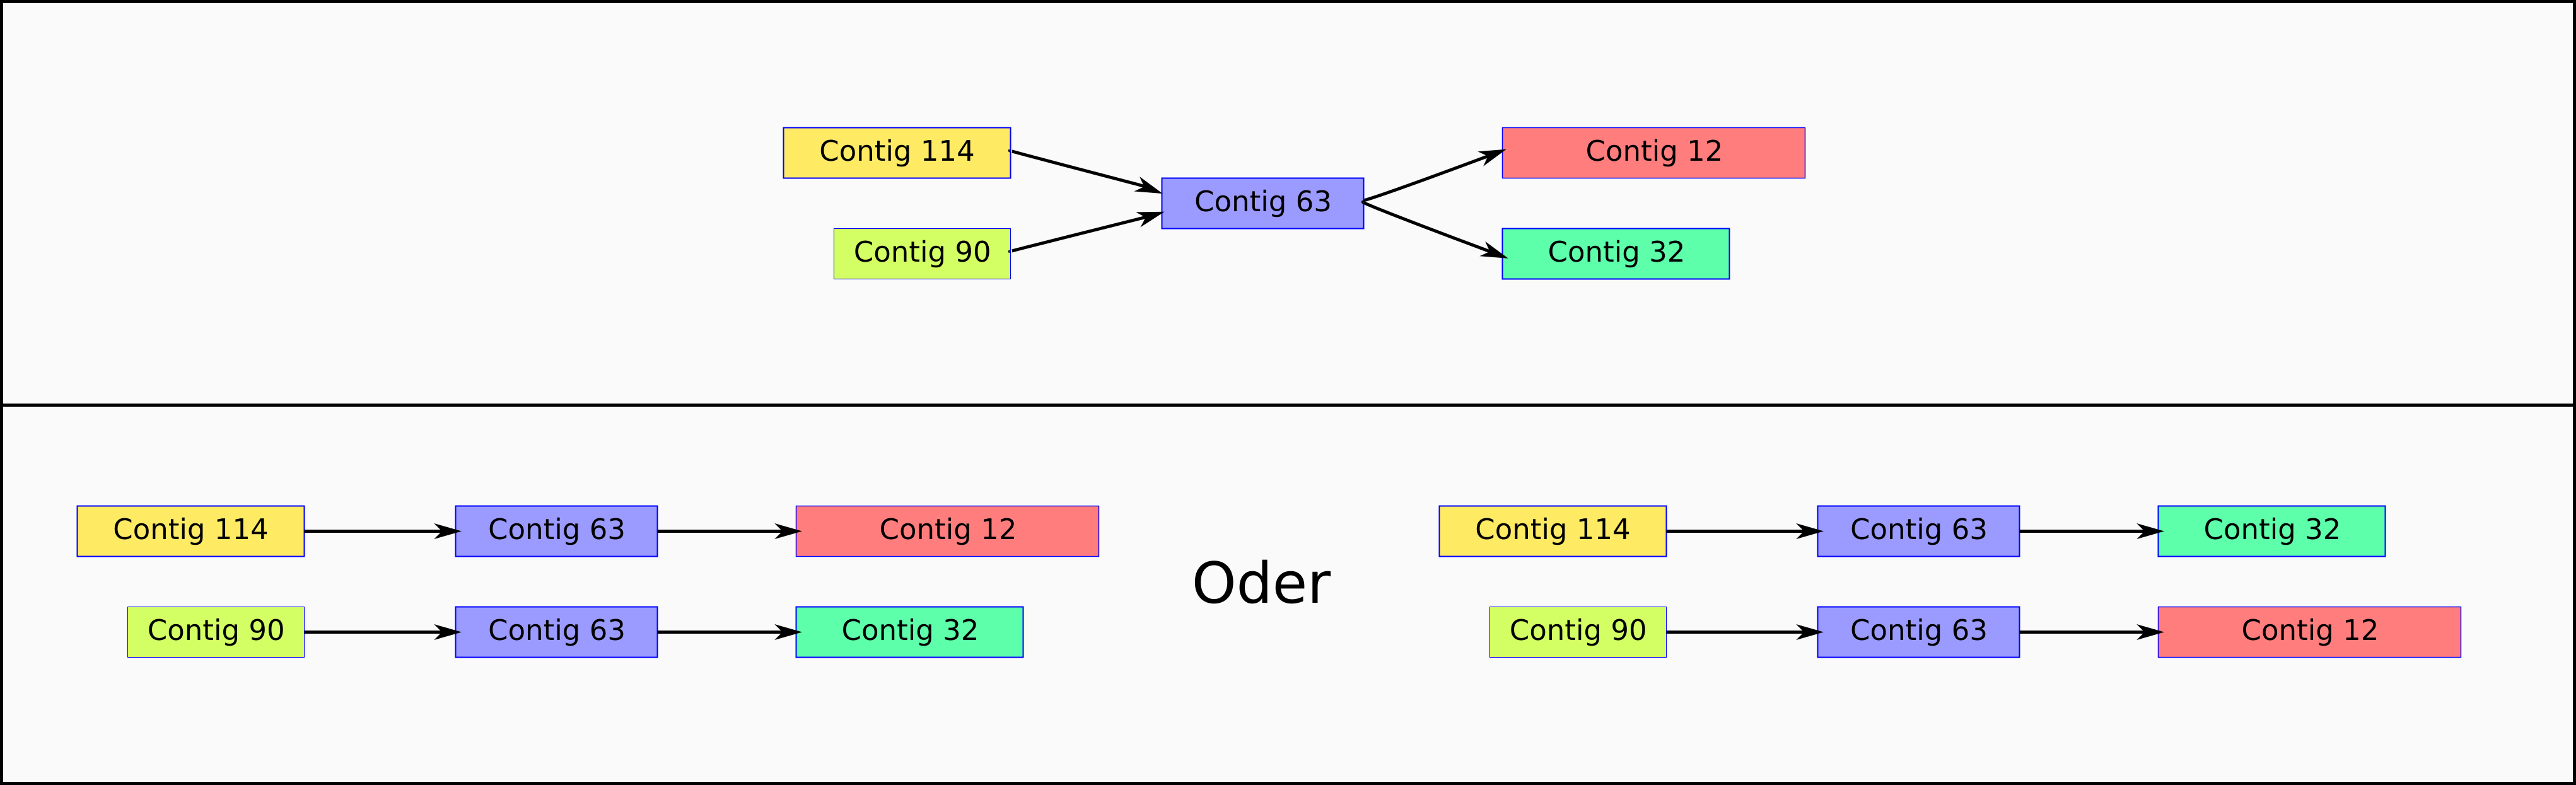
\includegraphics[width=0.9\textwidth]{bilder/repeat}
\end{center}
\caption{Repeat in einer Sequenz}
\label{repeat}
\end{figure}



Noch größere Schwierigkeiten machen eine andere Form von repetitiven Regionen in der DNA, bei denen sich zwei Regionen gleichen, welche 
%A19: sich eingefügt
sich in unterschiedlichen Bereichen in dem Strang befinden. Das Problem dieser Repeats wird in Abbildung \ref{repeat} verdeutlicht. 
%Noch größere Schwierigkeiten machen Regionen in der DNA, die über eine längere Strecke komplett identisch sind, sogenannte Repeats. Das Problem wird in Abbilding \ref{repeat} verdeutlicht. 
Zu sehen sind fünf Contigs, wobei ein Pfeil von Contig $a$ zu Contig $b$ bedeutet, dass in der DNA Contig $a$ direkt vor Contig $b$ kommt. Da Contig 63 (blau) zwei mal in der DNA vorkommt, ist es nicht trivial zu bestimmen, wie der Strang verläuft. 
% A19: Und 
Ferner ist MHC sehr repetitiv, somit werden viele Contigs mehrfach in der Sequenz auftauchen. Daher reichen die Daten aus Illumina nicht aus
%A19: Komma 
, um MHC zu assemblieren.


Eine weitere Möglichkeit der Sequenzierung ist die 
% A19: emph ergänzt 
\emph{Nanopore-Sequenzierung} \cite{Nanopore}. Hierbei können sehr lange Reads von 10\,000 bis über 1\,000\,000 Basenpaaren gelesen werden. Aufgrund des Längenunterschieds werden die Reads aus der 
% A19: Illuminar Sequenzierung 
Illumina-Sequenzierung auch \emph{Short-Reads} genannt 
% A19: ,
und die Reads aus der Nanopore-Sequenzierung \emph{Long-Reads}. Durch ihre Länge umfassen die Long-Reads oftmals bereits vollständige Repeats plus Umgebung. In 
% A19: unserer 
Abbildung \ref{repeat} entspräche dies einem Read, in dem Contig 114, Contig 63 und Contig 32 (gelb, blau und grün) Teil von einem Read sind und es keine Schwierigkeiten diesbezüglich gibt. Leider ist die Fehlerrate bei dieser Methode sehr hoch \cite{Harris475194}. 
So werden sehr viele Long-Reads aus der selben Region benötigt, um die richtigen Basenpaare einigermaßen verlässlich zu bestimmen.


Daher hat die Manchot-Forschungsgruppe vom Institut für Medizinische Mikrobiologie und Krankenhaushygiene der HHU, mit deren Zusammenarbeit diese Arbeit entstand, eine Kombination der beiden Methoden entwickelt.
Die verlässlichen Contigs aus der 
Illumina-Sequenzierung wurden auf die Long-Reads gemappt und so deren Abstände zueinander bestimmt. 
Wir betrachten zur Anschauung Abbildung \ref{longread} eines Long-Reads. Die bunten Bereiche stellen Gebiete dar, in denen die Basenpaarsequenzen mit denen eines Contigs aus den 
Illumina-Daten übereinstimmen. In der selben Situation wie in Abbildung \ref{repeat} hätten wir nun die Information erhalten, dass Contig 114 und Contig 32 zusammengehören, also die rechte Auflösung des Graphen aus Abbildung \red{repeat} richtig ist.
\begin{figure}[b!]
\begin{center}

\includegraphics[width=0.8\textwidth]{bilder/longread}
\end{center}
\caption{Ein Long-Read über mehrere Contigs}
\label{longread}
\end{figure}
% A19: Absatz machen

Die Manchot-Forschungsgruppe hat diese Daten gesammelt und daraus eine Liste aus paarweisen Daten extrahiert. Diese besitzt die Form: Contig $a$ hat zu Contig $b$ die Entfernung $d$ (in Anzahl von Basenpaaren zwischen $a$ und $b$). Dieses Dreiertuple aus zwei Contigs und einer Distanz nennen wir einen \emph{Constraint}.


Es bleiben noch einige Schwierigkeiten für die Assemblierung zu beachten. Die Distanzwerte zwischen den Contigs sind meistens durch Fehler in den Long-Reads verfälscht. Dadurch sind erst mehrere Constraints, die eine ähnliche Distanz zwischen zwei Contigs prognostizieren, wirklich belastbar. Bis zu welcher Distanz sich Constraints noch bestätigen und ab wann sie sich widersprechen ist hierbei ein entscheidender Aspekt, der betrachtet werden muss. Die Repeats lassen sich nicht immer so eindeutig auflösen wie in unserem Beispiel. In manchen Fällen kann erst im Gesamtzusammenhang erkannt werden, wie der Strang verläuft. Letztlich bleibt noch die große Datenfülle als Herausforderung zu nennen: Bei rund 122\,000 auftretenden Distanzen zwischen 2\,124 Contigs ist eine manuelle Zusammenfügung nicht zielführend und mindestens eine Teilautomatisierung der Prozesse obligatorisch. Auf der anderen Seite sind die Constraints nicht gleichmäßg verteilt, sodass es Regionen gibt, bei denen mit sehr wenig Informationen ausgekommen werden muss.

Hier stellt sich die Frage, mit welchen Methoden diese Probleme bewältigt werden können. Denkbar wäre eine Umsetzung mittels 
% A19 : emph ergänzt
\emph{Linearer Programmierung}. Das Ziel dieser Arbeit wird sein, zu untersuchen, ob lineare Programmierung hierbei anwendbar ist
% A10: ,
 und welche Vor- und Nachteile lineare Programme mit sich bringen.



\chapter{Formalisierung}\raggedbottom 

Die vorliegenden Daten der Manchot-Forschungsgruppe bestehen aus zwei Dateien: 
\begin{enumerate}
	\item einer Liste von allen Contigs und deren Länge gemessen in der Anzahl an Basenpaaren, die im Contig auftreten
	\item einer Datei mit den eingangserwähnten Constraints.
\end{enumerate}
Letztere besitzt folgenden dreispaltigen Aufbau:
\begin{align*}
&a \quad b \quad 1000\\
&a \quad b \quad 1100\\
&b \quad c \quad 3000\\
&a \quad c \quad 6000
\end{align*}


Dabei entspricht jede Zeile einem Constraint. Die ersten beiden Zeilen geben jeweils die beiden involvierten Contigs an. In der dritten Spalte sind die gemessenen Distanzen angegeben. Diese sind als Entfernung vom rechten Rand des ersten Contigs zum linken Rand des zweiten Contigs in Basenpaaren zu interpretieren. Negative Distanzen sind auf Überlagerungen einzelner Contigs zurückzuführen. Durch Hinzunahme der Längen der Contigs lassen sich die Distanzen auch so modifizieren, dass sie den Abstand der ersten Basenpaare der jeweiligen Contigs angeben. Im Folgendem werden wir nur noch die so modifizierten Distanzwerte verwenden. Zusätzlich zu den Constraints aus den Long-Reads stammen etwa 2\% der Constraints direkt aus der Illumina Sequenzierung. Hier wurde mehrmals die Distanz zwischen 
% A19: benachbarte 
benachbarten Contigs gemessen und der Durchschnitt daraus berechnet. Dadurch können auch nicht ganzzahlige Werte als Distanzen auftreten.

Wir werden im folgenden oft eine graphentheoretische Darstellung der Daten verwenden. Dabei sind die Contigs Knoten in einem Multigraphen und ein Constraint $(a,b,d)$ 
% A19 : eine -> entspricht einer
entspricht einer 
% A19:gerichtete 
gerichteten Kante von $a$ nach $b$ mit Länge $d$ als Attribut. Dabei werden die Begriffe Contig und Knoten sowie Constraint und Kante synonym verwendet
% A19: : „Nachfolger eines Contigs“, „ausgehender Constraint“.
. Daraus resultieren Begrifflichkeiten wie etwa „Nachfolger eines Contigs“ und „ausgehender Constraint“.

Zu einer gegebenen Positionierung ist der Fehler eines Constraints gegeben durch den Unterschied von der Distanz in der Positionierung zu der Distanz im Constraint. Wenn also Contig $a$ 300 Basenpaare vor Contig $b$ positioniert wurde, dann haben die beiden Constraints $(a,b,200)$ und $(a,b,400)$ beide einen Fehler von 100.
Ein Constraint ist durch eine Positionierung erfüllt, 
% A19:bzw 
beziehungsweise eine Positionierung von einem Constraint bestätigt, wenn der Fehler des Constraints kleiner als ein Schwellenwert ist, der im Laufe des folgeden Abschnittes festgelegt wird.
\section{Anforderungen an die Lösung}
Nun wollen wir einige Gütekriterien für mögliche Lösungen festlegen, um während der Bearbeitung Orientierungspunkte für die weitere Optimierung des Algorithmus zu haben und um diesen nach Abschluss anhand dieser Kriterien zu bewerten.
Folgende Punkte sollen beachtet werden:
\begin{enumerate}
	\item Wenn mehr als zwei Constraints eine ähnliche Distanz zwischen zwei Contigs 
	% A19: sieht, sollten
	implizieren, sollte die Lösung diese Distanz möglichst gut erfüllen.
	\item Ein Großteil der restlichen Constraints sollte auch zu der Positionierung passen.
	\item Es sollten möglichst wenig Contigs nahe zueinander positioniert werden, die keine gemeinsamen Constraints aufweisen. Diese Situation wird durch Abbildung \ref{gespallten} illustriert. Der obere Teilabschnitt zeigt eine Lösung, bei der die Bedingung nicht erfüllt wurde. Realistischer ist jedoch, dass hierbei ein Teilblock bestehend aus Contig 12 und Contig 32 doppelt in dem DNA-Strang vorkommt und bei der Lösung des Problems zwei separate Stränge ineinander verflochten wurden. Dies ist in der unteren Bildhälfte dargestellt.
	
	\begin{figure}
		\begin{center}
			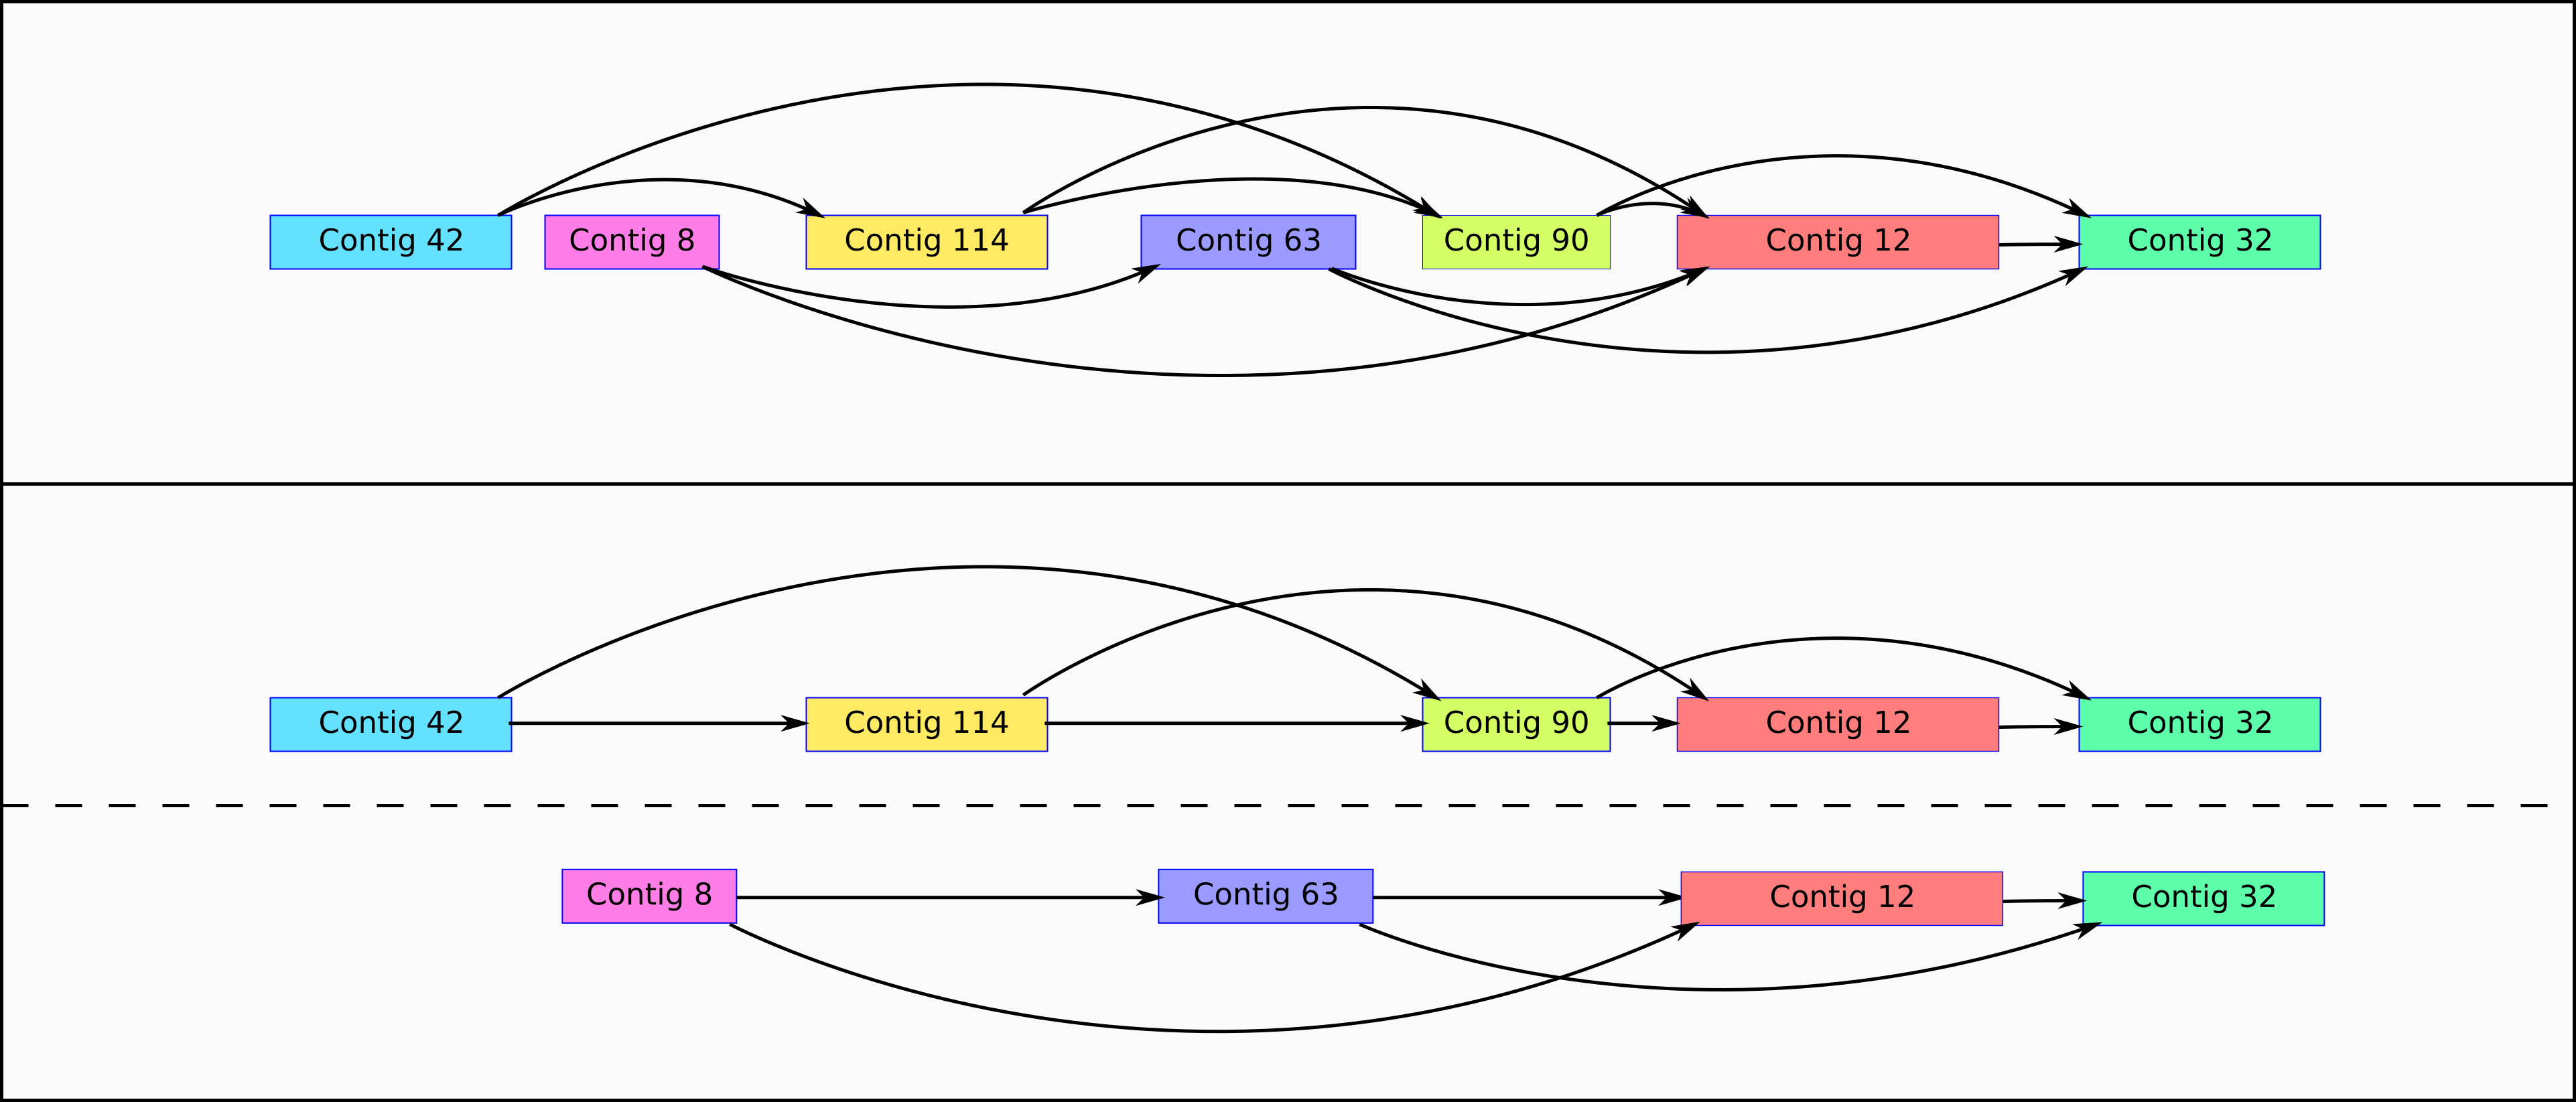
\includegraphics[width=1\textwidth]{bilder/gespallten}
		\end{center}
		\caption{Verflochtene Stränge}
		\label{gespallten}
	\end{figure}
	
	\item Die Entfernung vom ersten zum letzten Contig sollte zwischen 4,8 Millionen und 5 Millionen Basenpaare lang sein, da dies die ungefähre Gesamtlänge des Strangs ist.
	\item Bei einer Lösung wäre es zudem gut, wenn man Informationen darüber besitzen würde, wie wahrscheinlich es ist, ob verschiedene Teilgebiete tatsächlich so im Strang auftreten. Dabei wäre zum Beispiel eine Unterteilung in „sichere“ und „unsichere“ Gebiete interessant.
\end{enumerate}

Nun wollen wir konkretisieren, bis zu welchem Abstand Constraints ähnliche Distanzen haben. Dazu betrachten wir, wie die Standardabweichung der Distanzen von Constraints verteilt ist.
In der Abbildung \ref{std} werden die zu einem Basenpaar zugehörigen Constraints gegen ihre Standardabweichung geplottet. 
Dabei wurden pro Basenpaar die jeweiligen Distanzen der Constraints zu einer (Multi-)Menge zusammengefasst. Es wurde symmetrisch vorgegangen, das heißt Paare der Form (a,b) und (b,a) werden in der gleichen Menge behandelt. Ferner wurden Mengen mit einem Element nicht berücksichtigt, da es hier keine Abweichung gibt. Für die jeweiligen Mengen wurden dann die Standardabweichungen berechnet, der Größe nach geordnet und dann mit Berücksichtigung dieser Ordnung geplottet.
Der Plot wird mit zwei Skalierungen angegeben: Auf der linken Seite sieht man eine logarithmische Skalierung, während der rechte Plot eine lineare Skalierung verwendet.

\begin{figure}
	\begin{center}
		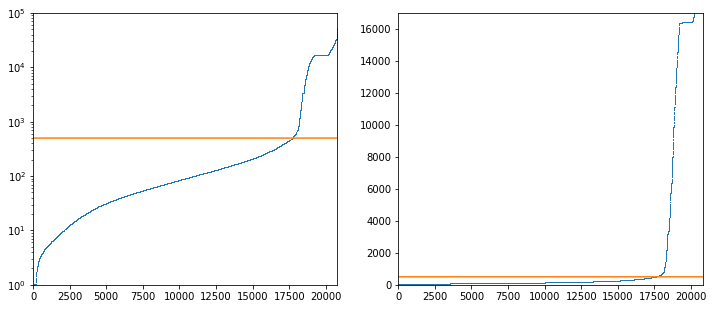
\includegraphics[width=0.8\textwidth]{bilder/std}
	\end{center}
	\caption{Standardabweichung der Distanzwerte}
	\label{std}
\end{figure}




Eine optische Betrachtung der Plots legt folgende Interpretation nahe: 
Es gibt einen Bereich der natürlichen Abweichung in der Datenmenge. Dies entspricht dem relativ flachen Anfangsbereich des Graphen. Ab einem gewissen Punkt "explodieren" die Werte. Hier ist die Standardabweichung innerhalb der Constraints so hoch, dass man nicht mehr von natürlicher Abweichung innerhalb der Daten ausgehen kann. Die orangene Linie grenzt diese Bereiche intuitiv voneinander ab. 
Diese liegt bei einer Standardabweichung von 500 Basenpaaren. 
Somit unterstützen sich Constraints, deren Distanzwerte sich nicht um mehr als 500 Basenpaare unterscheiden.

Um die oben genannten Forderungen an eine Lösung zu erfüllen, ist es notwendig die Repeats auszumachen und die Constraints auf diese Repeats aufzuteilen. Dazu halten wir uns an das Prinzip: „so viel wie nötig, so wenig wie möglich“.
Um dies sicherzustellen, sollte ein Contig, der mehrfach in der DNA vorkommen soll, zwei Punkte für jede seiner Versionen erfüllen:

\begin{enumerate}
	\item Es sollte mindestens ein Contig in der Nachbarschaft liegen, zu welchem es drei oder mehr Constraints gibt.
	\item Er sollte zu seinem direkten Vorgänger und Nachfolger im Strang mindestens ein Constraint aufweisen.
	%\item Es sollte ein Constraint zu einem Contig geben, der nicht selbst ein Repeat ist.
\end{enumerate}
Der erste Punkt soll sicherstellen, dass es nicht einfach ein Fehler in den Daten ist. Der zweite Punkt stellt sicher, dass der richtige Contig als Repeat markiert wurde. Wenn der Distanzwert eines Constraints nicht erfüllt ist, ist erstmal nicht klar, welcher der beiden beteiligten Contigs eine Repeat-Version haben soll. Der dritte Punkt stellt sicher, dass ein Contig nicht zu einer Repeat-Region hinzugefügt wird, in der er nicht gehört.

% Gebiete anders zueinander stehen, als sie es gerade tun, so ist nicht klar welche der beiden Gebiete ein Repeat besitzt. Daher ist es Sinnvoll dass die Repeatversion Constraints zu beiden Seiten haben muss, um sich in den Strang zu integrieren.
%Denn wenn viele Constraints zwischen zwei Gebiete nahlegen, dass diese Gebiete anders zueinander stehen, als sie es gerade tun, so ist nicht klar welche der beiden Gebiete ein Repeat besitzt. Daher ist es Sinnvoll dass die Repeatversion Constraints zu beiden Seiten haben muss, um sich in den Strang zu integrieren.
\chapter{Das lineare Programm}
\section{Eine kurze Einführung}
Die Problemstellung in dieser Arbeit lässt sich als lineares Programm (kurz LP) formulieren. In der linearen Programmierung möchten wir, unter Berücksichtigung von linearen Nebenbedingungen an die Funktionsparameter, eine lineare Funktion maximieren oder minimieren.
Formal mathematisch lässt sich der Minimierungsfall so fassen:
\begin{align*}
Gegeben:&\quad c \in \mathbb{R}^{n},\ A \in \mathbb{R}^{n \times m},\ b \in \mathbb{R}^{m} \\
Gesucht:&\quad \argmin_{ x\in \mathbb{R}^n}\{c^Tx\,|\, Ax \leq b\}
\end{align*}
Dabei wird folgende Notation verwendet:
\begin{description}
	\item[\quad Variablen] $x_1,..., x_n$
	\item[\quad Zielfunktion]  $c^Tx = \sum_{i=1}^n c_i x_i$
	\item[\quad Nebenbedingungen]  $Ax \leq b \ \Leftrightarrow\ \sum_{i=1}^n a_{ji} x_i \leq b_j, \ j = 1,...,n$
\end{description}
Lineare Programme lassen sich in Polynomialzeit berechnen. Daher eignen sie sich oft als Werkzeug für verschiedenste Probleme. 
Weitere Informationen zur Linearen Programmierung findet man in \cite{bertsimas1997introduction} und \cite{schrijver1998theory}.
Es ist auch möglich, den Definitionsraum der Variablen (teilweise) auf ganze Zahlen zu beschränken. Dies bezeichnet man dann als ein ganzahliges lineares Programm (kurz ILP). ILPs bieten einige Möglichkeiten die mit LPs nicht umzusetzen wären. Sie sind dafür aber NP-schwer und somit wahrscheinlich nicht polynomialzeitberechenbar. Eine Einschränkung des Problems ist eines der 21 NP-vollständigen Probleme von Karp \cite{karp1972reducibility}. Die NP-Schwere von divers Modifikationen wird zudem in \cite{schrijver1998theory} bewiesen.

\section{Assembly als LP}
Im Folgenden bezeichnet $C$ die Menge aller Contigs und $D$ die Multimenge aller Constraints. Dabei wurde der Distanzwert jedes Constraints in $D$ so umgerechnet, dass er die Entfernung 
% A19: von 
vom linken Rand 
% A19: vom 
des ersten Contigs bis zum linken Rand des zweiten Contigs angibt.
Wir möchten die Contigs so positionieren, dass der durchschnittliche Fehler aller Constraints 
% A19: möglich 
möglichst klein ist. Als Formel:
\[ \pos = \argmin_{\pos\,:\, C \rightarrow \mathbb{N}} \ \sum_{(a,b,\delta) \in D} |\pos(b) - \pos(a) - \delta| \] 
Um daraus ein lineares Programm zu machen, führen wir für jeden Constraint $(a,b,\delta)$ aus $D$ eine Hilfsvariable $\varepsilon$ ein:
\[ \varepsilon = |\pos(b) - \pos(a) - \delta| \]
Mit Hilfe dieser Variablen können wir die zu minimierende Zielfunktion wie folgt darstellen:
\begin{align*}
\quad& \sum_{d \in D} \varepsilon_{d}
\end{align*}
Nun müssen wir noch die Informationen über die Fehler, also $\varepsilon = |\pos(b) - \pos(a) - \delta|$, einbauen. Da wir ohnehin die Summe der Fehler minimieren wollen, ist es ausreichend, folgende Ungleichung zu fordern:
\begin{align*}
\varepsilon \geq |\pos(b) &- \pos(a) - \delta|
\end{align*}
Dies liegt daran, dass bei Minimierung immer die untere Schranke angenommen wird, welche in diesem Fall die Gleichheit ist. Nun ist die Betragsfunktion aber nicht linear. Sie lässt sich aber äquivalent durch die folgenden beiden linearen Ungleichung darstellen:
\begin{align*}
\pos(b) - \pos(a) - \delta &\leq \varepsilon\\
-\pos(b) + \pos(a) + \delta &\leq \varepsilon
\end{align*}

Zusammengefasst erhalten wir also folgendes lineares Programm für die Berechnung der optimalen Positionierung:

\begin{align*}
\text{Variablen:}\quad& \pos(c) \ \forall c \in C \ \ \text{und} \ \ \varepsilon_{d} \ \forall \ d \in D\\
\text{Zielfunktion:}\quad& \sum_{d \in D} \varepsilon_{d}\\
\text{Bedingungen:}\quad \begin{split} \pos(b) - \pos(a) - \delta \leq \varepsilon_{d}\\
-\pos(b) + \pos(a) + \delta \leq \varepsilon_{d} \end{split}\quad \forall \ (a,b,\delta) = d \in D
\end{align*}
Distanzwerte weisen zu große Schwankungen auf, um auf ein Basenpaar genau zu sein. Daher bietet es sich an, die Relaxierung des LPs zu betrachten, also auch reelle Positionen zuzulassen. Durch diese Lockerung der Bedingungen lässt sich das Programm wesentlich schneller lösen.

Dieses LP sorgt nur dafür, dass die Constraints möglichst gut erfüllt sind. Weder verhindert es, dass Contigs, welche keine Constraints vorweisen, nahe positioniert werden, noch erkennt es Repeats. Um das weitere Vorgehen planen zu können, bietet es sich trotzdem an, diesen Ansatz auszuführen und anhand der Lösung konkrete Problemstellen zu lokalisieren. 


Die Implementierung erfolgt in der Jupyter-Umgebung der Programmiersprache Python. Dabei wird Gurobi \cite{Gurobi}, 
% A19: einem 
ein Programm
% A19: Komma
, das auf mathematische Optimierung spezialisiert ist, verwendet. Das Programm liefert uns als Rückgabe eine konkrete Positionierung der Contigs. Nun wäre es gut, wenn wir eine Möglichkeit hätten, festzustellen, inwiefern die von uns festgelegten Kriterien erfüllt sind. Im nächsten Kapitel werden dazu verschiedene optische Verfahren diskutiert.

%Somit lässt es sich nur unterstützend einsetzen. Wie mit Hilfe von ILPs auch diese beiden Punkte abgedeckt werden könnten, diskutieren wir im letzten Kapitel.



\chapter{Wie man eine Lösung grafisch darstellt}
Ein wichtiger Aspekt für die Arbeit mit großen Datenmengen ist die Visualisierung.
Sie sollte in der Lage sein, die wichtigsten Informationen auf einen Blick sichtbar zu machen. Wir beschäftigen uns nun mit Möglichkeiten, konkrete Positionierungen der Contigs, also Abbildungen $pos: C \rightarrow \mathbb{R}$, zu visualisieren.
Eine erste, naheliegende Option ist eine lineare Darstellungsweise. Hierbei werden die einzelnen Contigs gemäß ihrer Positionierung und ihrer Länge auf der reellen Zahlengerade eingezeichnet. Um Überlappungen zu beachten, bietet es sich an, mehrschichtig zu arbeiten. Mehrschichtig bedeutet hier, dass bei Überlappung zweier Contigs der hintere Contig in einer anderen Höhe geplottet wird. Diese Methode wird durch Abbildung \ref{plot1} illustriert.
Vorteile dieser Darstellungsweise sind unter anderem die folgenden Aspekte:
\begin{figure}
	\begin{center}
		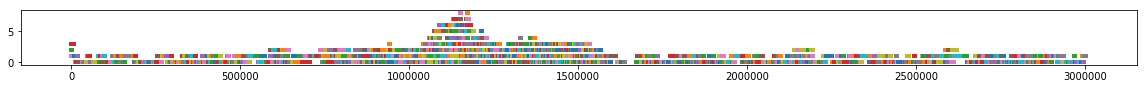
\includegraphics[width=17cm]{bilder/plot1}
	\end{center}
	\caption{Linearer Plot vom Ergebnis des ersten LPs}
	\label{plot1}
\end{figure}
\begin{enumerate}
	\item Der gesamte Strang inklusive seiner Länge ist auf einen Blick sichtbar. Dies liefert dem Betrachter einen groben Überblick. Ferner lässt sich der fünfte Unterpunkt der Anforderungen an Lösungen, die Länge des Stranges, so auch optisch leicht überprüfen.
	%\item Durch das mehrschichtige Arbeiten lassen sich Regionen mit einer hoher Überlappungsdichte (also hoher Coverage) leicht lokalisieren.
	\item Regionen, die hauptsächlich aus großen oder aus kleinen Contigs bestehen, lassen sich anhand des Plots leicht lokalisieren. Für den fünften Unterpunkt unsere Anforderungen an eine Lösung lässt sich dies als Indiz für die Sicherheit dieser Umgebungen verwenden. In Gebieten, in denen nur wenige, aber große Contigs vorkommen, sollten im Schnitt weniger Fehler hinsichtlich der geringeren Datenmenge auftreten als in mit vielen kleinen Contigs überfüllten Regionen.
	\item Durch Hinzunahme von Färbungen ist es möglich, einige Kerninformationen leicht zugänglich zu machen. Dazu zählen etwa die Anzahl der Repeats eines einzelnen Contigs oder der Gesamtanteil an sich wiederholenden Contigs.
\end{enumerate}
Jedoch gibt es einen zentralen Nachteil bei der Wahl dieser linearen Darstellungsform: Die Information, die wir durch die Constraints erhalten, werden in der Visualisierung nicht berücksichtigt.
Damit lässt sich die Einhaltung der ersten drei Kriterien an eine Lösung optisch nicht analysieren.
Beispielsweise sieht man nicht, ob benachbarte Contigs auch tatsächlich gemeinsame Constraints aufweisen.
Um auch die Constraints mit einzubeziehen, bedarf es einer weiteren Darstellungsweise.

Um auch die Constraints mit einzubeziehen, bedarf es einer weiteren Darstellungsweise.
Ähnlich wie in Abbildung \ref{gespallten} lassen sich dafür gerichtete Graphen verwenden. Dabei bildet die Menge der Contigs die Knoten des Graphen. Constraints zwischen zwei Knoten lassen sich als (gerichtete) Kanten darstellen.
Um eine gewisse Übersichtlichkeit zu erhalten, ist es aber sinnvoll, nicht alle Constraints zu plotten.
Stattdessen nutzen wir die gegebene Positionierung aus und zeichnen nur Kanten für nah beieinander positionierte Contigs mit gemeinsamen Constraints. % und Kanten welche besonders lang sind.
Dabei gehen wir für jeden auftretenden Contig $a$ wie folgt vor:
\begin{itemize}
	\item Zunächst werden alle Constraints gelöscht, deren Fehler in der vorgegebenen Positionierung größer als eine fixierte Konstante ist. Oftmals fällt die Wahl hier auf eine Zahl in der Größenordnung $500$ gemäß der Überlegungen bezüglich der Standardabweichungen in dem Kapitel der Formalisierung.
	\item Ferner werden mehrfach auftretende Constraints zusammengefasst und alle Schleifen, also alle Constraints der Form $(a, a, d)$ gelöscht.
	\item Sei nun $N_a$ die Menge aller Contigs, die zusammen mit $a$ in einem verbliebenden Constraint enthalten sind. Nun werden die Contigs in $N_a$ und $a$ selbst bezüglich ihrer Positionierung sortiert.
	\item Schließlich wird je eine Kante von $a$ zu den ersten beiden Contigs, die hinter $a$ positioniert wurden, gezeichnet. Umgekehrt wird je eine Kante von den ersten beiden Contigs, die vor $a$ positioniert wurden, zu $a$ gezeichnet.
	%\item Schließlich wird noch eine grün gefärbte Kante von $a$ nach $b$ gezeichnet, wenn es ein Constraint von $a$ nach $b$ aber weder ein Constraint von $a$ nach $c$ und von $b$ nach $c$ gibt, noch ein Constraint von $c$ nach $a$ und von $c$ nach $b$. 
	\item Zusätzlich werden noch grün gefärbte Kanten 
	% A19: gezeichnet 
	für alle Constraints gezeichnet, die nicht verlängerbar sind. Als verlängerbar gelten alle Constraints von $a$ nach $b$ und von $b$ nach $c$ für die es ein Constraint von $a$ nach $c$ gibt.
\end{itemize}
Im Allgemeinen tritt hierbei auch der Fall auf, dass eine Kante $(a,b)$ während des Prozesses doppelt eingezeichnet werden soll: Einmal im Durchgang von $a$ als auslaufende Kante und einmal im Durchgang von $b$ als einlaufende Kante.
Sie werden trotzdem nur einmal gezeichnet.

Die Wahl, dass jeder Knoten zwei Vorgänger und zwei Nachfolger bekommt, ist nicht fest, hat sich aber als besonders geeignet herausgestellt. Bei nur einem Vorgänger und einem Nachfolger kann es schnell passieren, dass ein eigentlich zusammenhängender Strang unzusammenhängend dargestellt wird. Abbildung \ref{t} illustriert diese Situation. Dabei entspricht die erste Abbildung der tatsächlich im Programm auftretenden Darstellungsform. In der zweiten Abbildung wurde die Situation noch einmal etwas schematischer skizziert und optisch mit Farben unterlegt.

Auch können mehrere Kanten interessante Einblicke über die Struktur geben. So gibt es Contigs, die nur eine einlaufende Kante besitzen oder deren Kanten mehrere Contigs überspringen. 
% A19: Alles 
Beides ist ein Zeichen von Unstimmigkeiten, die näher untersucht werden könnten.


\begin{figure}
	\begin{center}
		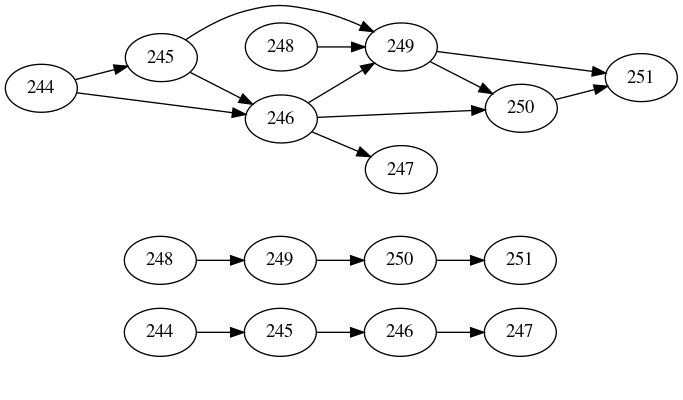
\includegraphics[width=6.6cm]{bilder/t}
		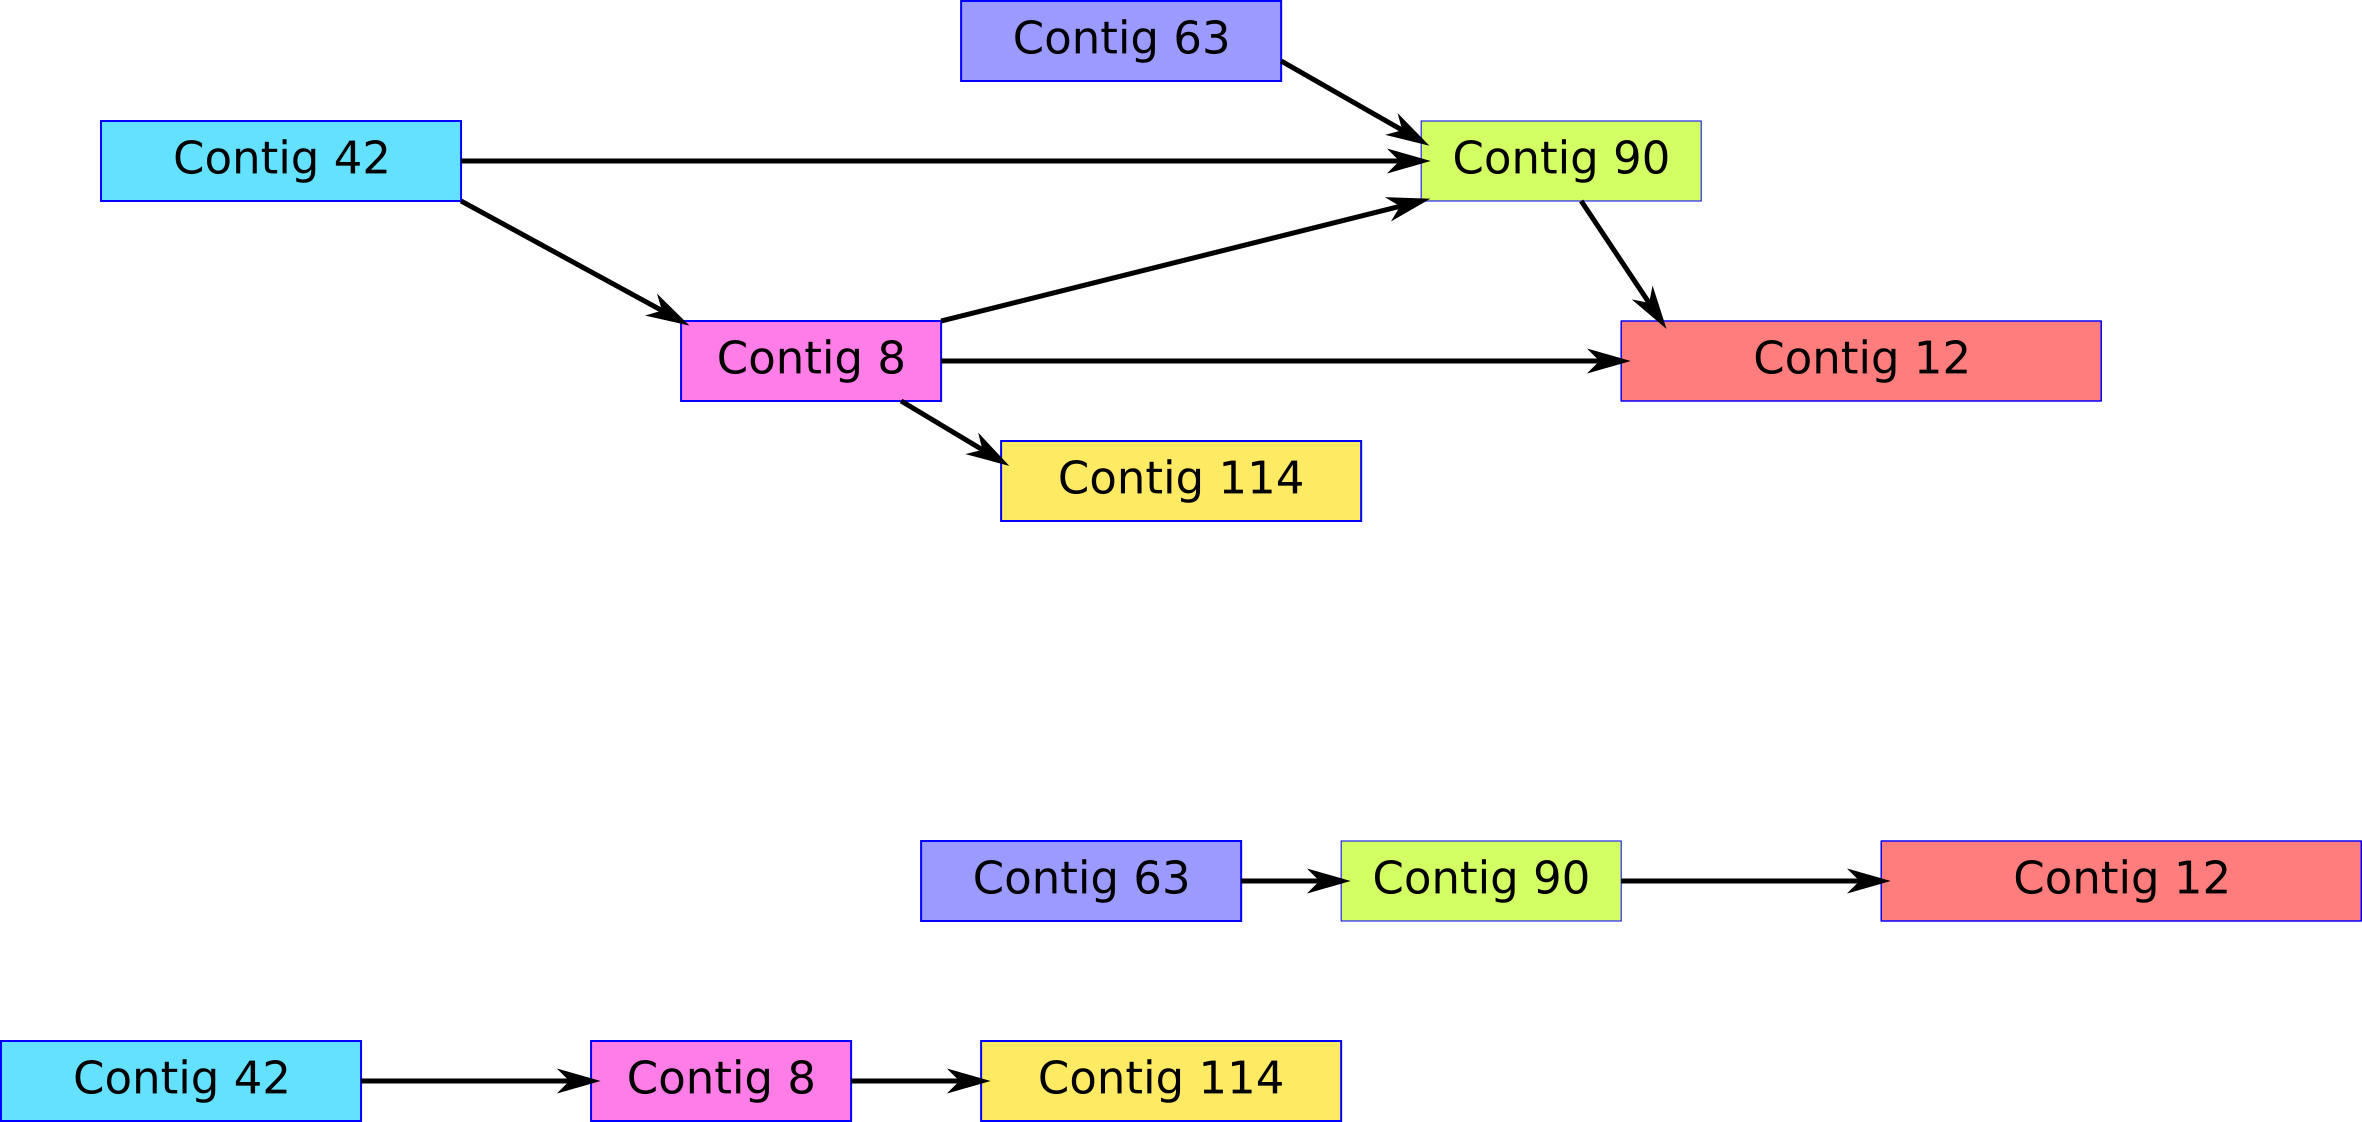
\includegraphics[width=6.6cm]{bilder/tt}
	\end{center}
	\caption{Probleme bei der optischen Darstellung mit nur einem Vorgänger und Nachfolger}
	\label{t}
\end{figure}


Wir betrachten nun das Ergebnis des Durchlaufs von unserem ersten LP. Dies wird in den Abbildungen \ref{plot1} und \ref{ersterdurchlauf} dargestellt. In beiden Plots fällt dem Betrachter direkt ein Ballungsräume auf. Ein Ausschnitt dessen ist in der zweiten Abbildung vergrößert dargestellt. An dieser Stelle hat das LP den Strang aufgerissen, um Repeats, welche hier noch als einzelner Contig auftreten, näher an entsprechende Nachbarn zu positionieren. Anhand des ersten, linearen Plots, sieht man zudem sofort, dass die Gesamtlänge des Strangs zu kurz ist.
Offenbar sind unsere Gütekriterien somit nicht erfüllt und es bedarf einer Modifikation des Verfahrens.


%Die grünen Kanten geben einen guten Überblick, wie weitläufig die Constraints in dem Bereich vernetzt sind. Lange grüne Kanten die sich weitläufig überschneiden zeugen von einem Sicheren Gebiet, wärend wenige kurze grüne Kanten sehr unsicher sind.
%TODO height=30cm
\begin{figure}
	\begin{center}
		
\includegraphics[width=6.6cm]{bilder/vergrossert}
	\end{center}
	\caption{Ergebnis des LPs}
	\label{ersterdurchlauf}
\end{figure}
%\newpage

%	\caption{Ergebnis}
%	\label{ersterdurchlauf}
%\end{figure}



%\begin{minipage}{0.5\textwidth}
%\begin{figure}
%	\begin{center}
%		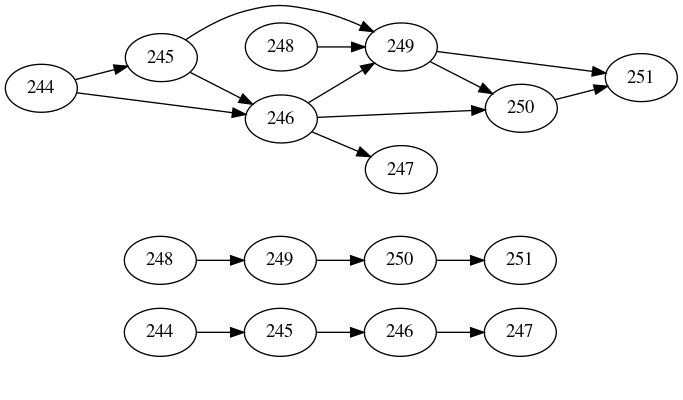
\includegraphics[width=0.9\textwidth]{bilder/t}
%	\end{center}
%	\caption{t}
%	\label{t}
%\end{figure}
%\end{minipage}

%\begin{minipage}{0.5\textwidth}
%\begin{figure}
%	\begin{center}
%		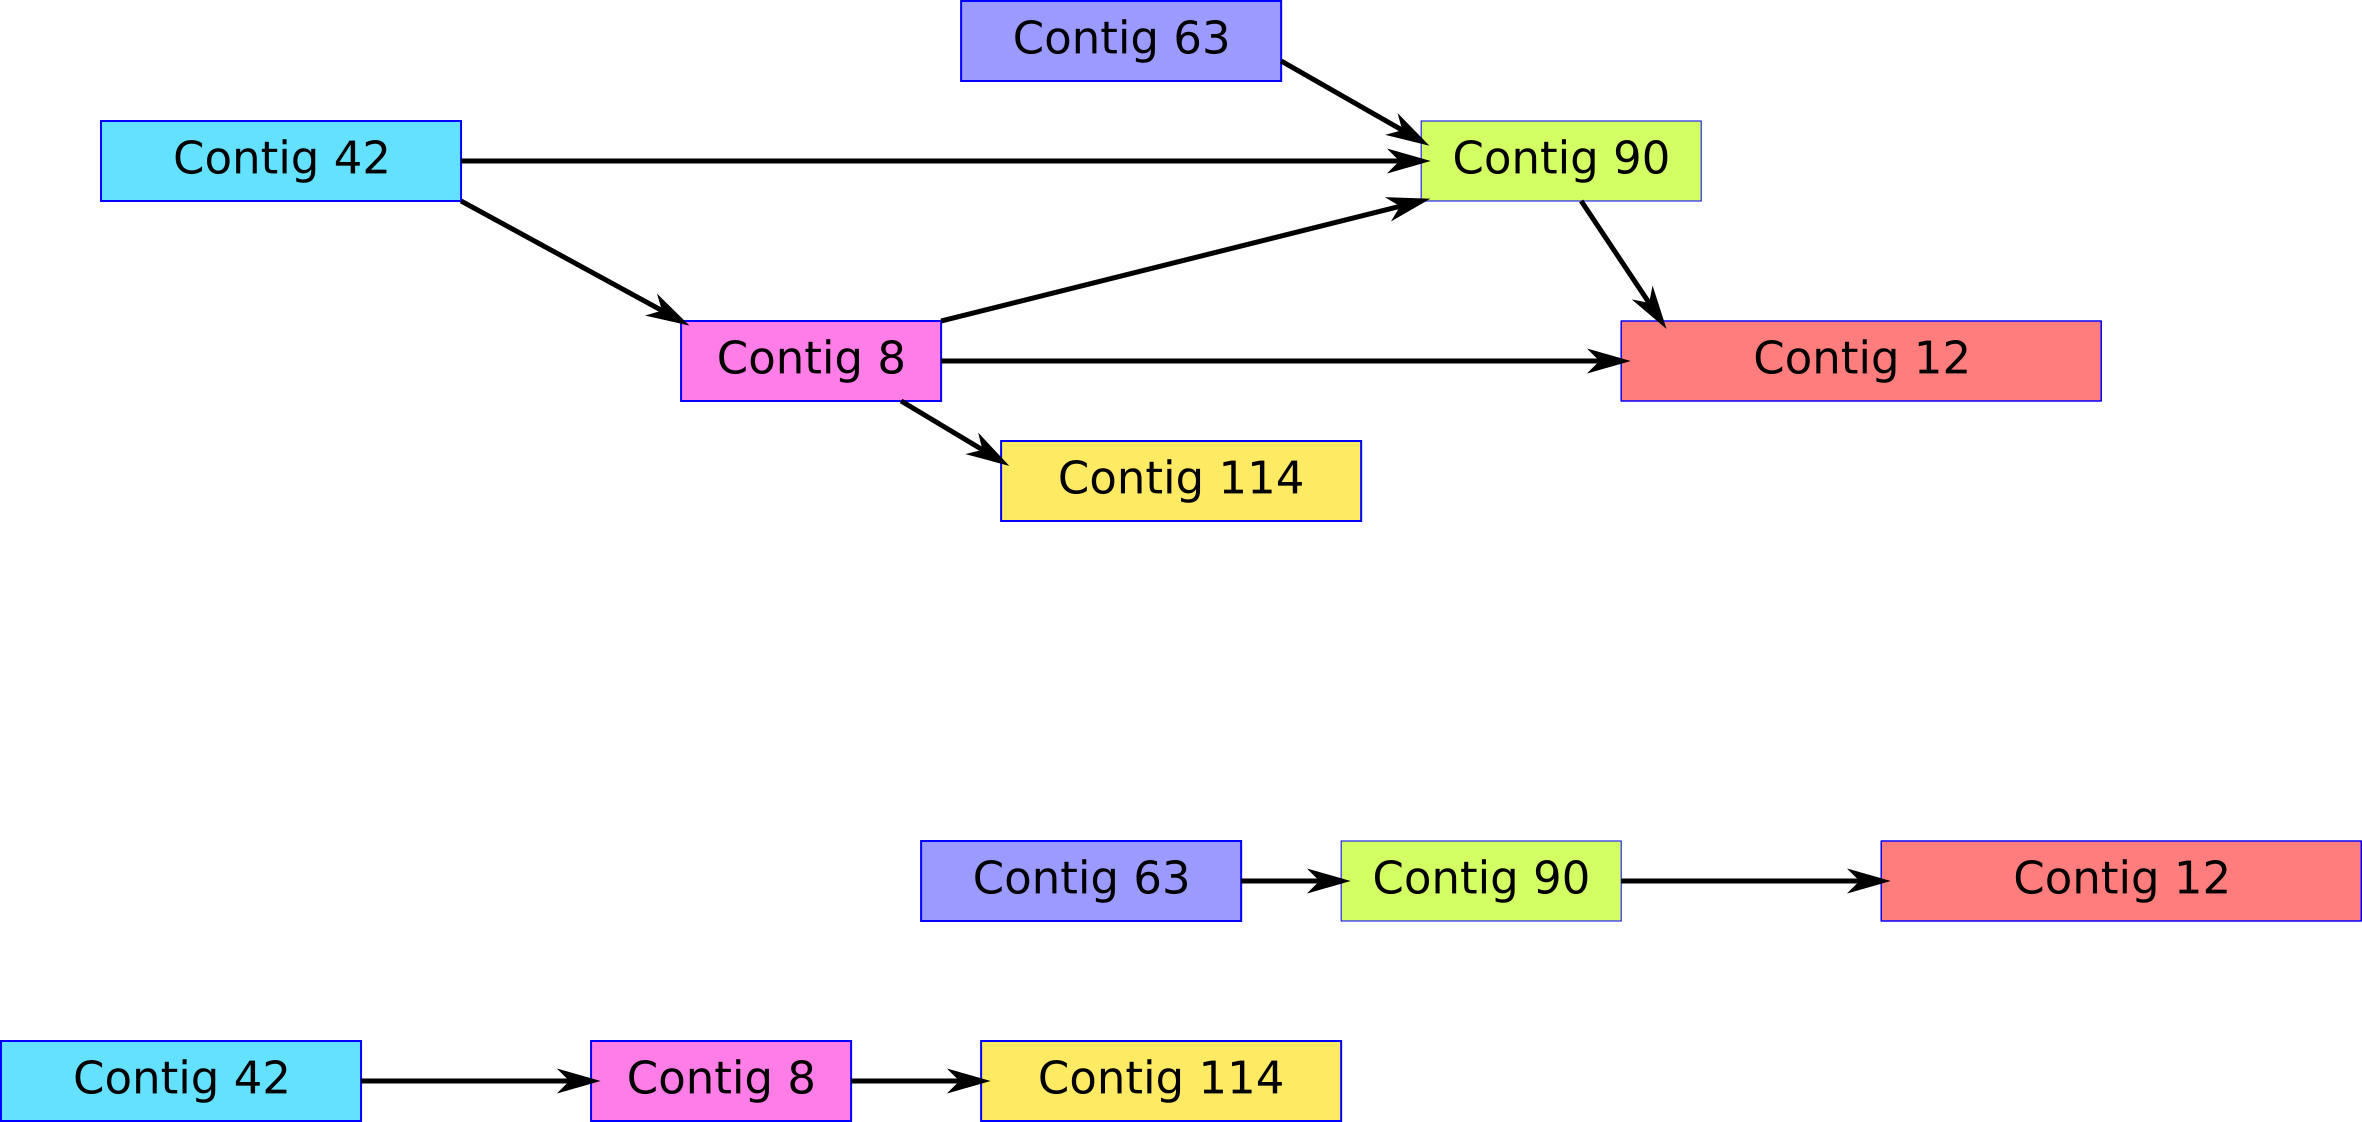
\includegraphics[width=0.9\textwidth]{bilder/tt}
%	\end{center}
%	\caption{tt}
%	\label{tt}
%\end{figure}
%\end{minipage}
\newpage
\chapter{Algorithmus Phase 1: Grobe Lösung aufbauen}

Am Ende des vorherigen Abschnittes haben wir festgestellt, dass eine einfache Ausführung des lineare Programmes nicht ausreicht, um eine Lösung zu konstruieren, die unsere Gütekriterien erfüllt. 
In dem Graphen, der zu der Lösung korrespondiert, erkennt man dies anhand der starken Verflechtung/Verknotung verschiedener Teilstränge. Um dies möglichst zu verhindern, gehen wir nun wie folgt vor:

Unser Ziel ist es, ein „Grundgerüst“ für eine fertige Lösung aufzubauen.
Dieses soll die Form eines Pfades von dem ersten bis zum letzten Contig des Stranges besitzen.
Dabei sollte der Pfad möglichst viele Contigs enthalten, welche zueinander richtig positioniert sind.
Es ist nicht notwendig, dass alle Contigs korrekt positioniert sind, da das lineare Programme vereinzelte Fehlpositionierungen der Contigs gut beheben kann. 


Wir speichern die Constraints als einen gerichteten Multigraphen $G$ aus der NetworkX Bibliothek \ref{}.
Für zeitintensivere Berechnungen, erstellen wir eine reduzierte Version $G_r$, in der ähnliche Kanten 
zu einer Kante wie folgt zusammengefasst werden:

Zunächst werden für je zwei Contigs alle Distanzwerte zwischen diesen beiden Contigs sortiert. Dabei betrachten wir für Contigs $a$ und $b$ sowohl Constraints der Form $(a, b, d)$ als auch der Form $(b, a, d)$. Allerdings fixieren wir eine Sortierung $(a, b)$ und negieren die Distanzwerte von $(b, a)$.Dann werden die Distanzwerte gruppiert, indem man die sortierten Distanzen als Folge betrachtet und immer eine Gruppe abspaltet, sobald sich zwei benachtbarte Werte um mehr als 500 Basenpaare unterscheiden. Jede Gruppe wird daraufhin zu einem einzelnen Constraint zusammengefasst, der den Median der auftretenden Werte als Distanz besitzt und mit der Gruppengröße gewichtet wird.

% A19: Gehen wir dies an einen kleinen Beispiel durch. Gegeben sind folgende Constraints zwischen zwei Contigs $a$ und $b$:
Das zuvor beschriebene Verfahren wird durch das folgende Beispiel verdeutlicht. Dabei sind die folgenden Constraints zwischen zwei Contigs $a$ und $b$ gegeben:
\begin{center}
	\begin{tabular}{lr}
		$a$\quad $b$\quad &100\\
		$a$\quad $b$\quad &11\,000\\
		$b$\quad $a$\quad &50\\
		$b$\quad $a$\quad &60\,000\\
		$a$\quad $b$\quad &70\\
		$a$\quad $b$\quad &300\\
		$a$\quad $b$\quad &10\,950\\
		$a$\quad $b$\quad &11\,050\\
		$a$\quad $b$\quad &20\\
		$a$\quad $b$\quad &600\\
		$b$\quad $a$\quad &200
	\end{tabular}
\end{center}
Die sortierten Distanzwerte:
\[-60000\ \ \,{-200}\ \ \,{-50}\ \ \,20\ \ \,70\ \ \,100\ \ \,300\ \ \,600\ \ \,10950\ \ \,11000\ \ \,11050\]
Gruppen bilden bei Abständen über 500:
\[-60000\,|\, {-200}\ \ \,{-50}\ \ \,20\ \ \,70\ \ \,100\ \ \,300\ \ \,600\, |\, 10950\ \ \,11000\ \ \,11050\]
Es resultieren diese drei Kanten in $G_r$:

\begin{center}
	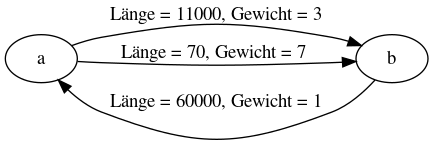
\includegraphics[width=0.4\textwidth]{bilder/dreikannten}
\end{center}


Unser Ziel ist es, einen Pfad durch $G$ vom ersten bis zum letzten Contig zu finden, der möglichst viele Contigs beinhaltet.
Dafür werden wir beim ersten Contig anfangen und uns schrittweise vorarbeiten. Sollte sich der Graph aufteilen, so versuchen wir zuerst mit Hilfe von Heuristiken zu bestimmen, welcher Pfad der Richtige ist. Sollte dies nicht möglich sein, werden alle Pfade ausprobiert.

Da das LP den Anfangs- und Endbereich gut lösen konnte, können wir den ersten und letztem Contig aus der Lösung ablesen. Dies sind Contig 2345APD und Contig 2080APD. Alle Contigs die nicht von 2345APD erreichbar sind oder die selbst 2080APD nicht erreichen können, werden für diese Phase nicht mehr betrachtet. Dies betrifft 21 der 2\,138 Contigs.

Wir beginnen also mit Contig 2345APD an Position 0. Für jede auslaufende Kante $e$ aus 2345APD wird zu dem Endknoten von $e$ die Länge der Kante in einer Liste gespeichert. Die Listen der ersten 10 Contigs sehen so aus: 

\begin{footnotesize}
	\begin{align*}
	\text{1483APD:}&\ 6632\ \ \,6662\ \ \,6662\\
	\text{1395APD:}&\ 6877\ \ \,6943\ \ \,6977\ \ \,6979\ \ \,6980\ \ \,6982\ \ \,6985\ \ \,6993\ \ \,6998\ \ \,6999\ \ \,7002\\
	\text{1596APD:}&\ 9809\ \ \,9867\ \ \,9903\ \ \,9931\ \ \,9939\ \ \,9942\ \ \,9951\ \ \,9978\\
	\text{2235APD:}&\ 14013\ \ \,14070\ \ \,14179\ \ \,14219\ \ \,14263\ \ \,14290\ \ \,14304\\
	\text{1534APD:}&\ 14687\ \ \,14732\ \ \,14841\ \ \,14930\ \ \,14957\ \ \,14972\\
	\text{546APD:}&\ 16242\ \ \,16254\ \ \,16372\ \ \,16470\ \ \,16550\\
	\text{577APD:}&\ 18659\ \ \,18782\ \ \,18967\ \ \,19040\ \ \,19081\\
	\text{998APD:}&\ 32244\ \ \,32453\\
	\text{209APD:}&\ 34061\ \ \,34257\\
	\text{1635APD:}&\ 43666
	\end{align*}
\end{footnotesize}

Es folgen noch 101 weitere Contigs mit jeweils nur einem Eintrag. 
% A19: Diese Werte werden wie bei der Erstellung des reduzierten Graphens gruppiert und Position der größten Gruppe den Contigs vorläufig zugeordnet. 
Für alle weiteren Contigs wird eine leere Liste erstellt.
Diese Werte werden analog zu der Erstellung des reduzierten Graphens listenweise gruppiert. Dann wird der Median der größten Gruppe dem Contig vorläufig als Position zugeordnet.

% A19: daraufhin ergänzt
Die Positionierung des Contigs mit der niedrigsten vorläufigen Position wird daraufhin fest gesetzt.
%der Contig mit der niedrigsten Position wird als nächstes gesetzt. 

Dies ist in diesem Fall Contig 1483APD an Position 6662. Auch von 1483APD werden die Distanzwerte der auslaufenden Kanten genommen. 
% A19: Diese werden aber zuerst zu seiner Position addiert und dann zu den schon bestehenden Werten von 2345APD hinzugefügt:
Um absolute Positionen (also relativ des Startcontigs) zu erhalten, addieren wir die Positionierung von 1483APD auf die Distanzen. Daraufhin werden diese neuen Positionen in den Listen ergänzt. Analog zum vorherigen Schritt werden nun wieder Gruppen und Mediane gebildet und schließlich eine weiter Positionierung eines Contigs fest gesetzt.

\begin{footnotesize}
	\begin{align*}
	\text{1395APD:}&\ 6877\ \ \,6943\ \ \,6977\ \ \,6979\ \ \,6980\ \ \,6982\ \ \,6985\ \ \,6993\ \ \,6998\ \ \,6999\ \ \,7002\quad\quad 6982\ \ \, 6989\ \ \,6994\\
	\text{1596APD:}&\ 9809\ \ \,9867\ \ \,9903\ \ \,9931\ \ \,9939\ \ \,9942\ \ \,9951\ \ \,9978\quad\quad 9906\ \ \,9946\\
	\text{2235APD:}&\ 14013\ \ \,14070\ \ \,14179\ \ \,14219\ \ \,14263\ \ \,14290\ \ \,14304\quad\quad 14109\ \ \,14308\\
	\text{1534APD:}&\ 14687\ \ \,14732\ \ \,14841\ \ \,14930\ \ \,14957\ \ \,14972\quad\quad 14771\ \ \,14976\\
	\text{546APD:}&\ 16242\ \ \,16254\ \ \,16372\ \ \,16470\ \ \,16550\quad\quad 16293\ \ \,16554\\
	\text{577APD:}&\ 18659\ \ \,18782\ \ \,18967\ \ \,19040\ \ \,19081\quad\quad 18698\ \ \,19044\\
	\text{998APD:}&\ 32244\ \ \,32453\quad\quad 32248\\
	\text{209APD:}&\ 34061\ \ \,34257\quad\quad 34065\\
	\text{1635APD:}&\ 43666
	\end{align*}
\end{footnotesize}

So wird der Strang Contig für Contig aufgebaut. Wir sammeln die bereits fest positionierten Contigs in einer Menge $P$ und die vorläufig positionierten Contigs in einer Menge $P_V$. % Der einfachheitshalber führen wir folgende Notation ein: Sei $c \in P$, dann ist $P[c]$ die Position des Contigs $c$, analog für $c \in P_V$. 
Den zuletzt in $P$ hinzugefügten Contig bezeichnen wir mit $a^*$.
Die Nachfolger von $a^*$, die bereits in $P$ sind, werden 
nur erneut aufgenommen, wenn die neue Position mehr als 10\,000 Basenpaare von der alten entfernt ist und die zugehörige Kante von $a^*$ zum Nachfolger im reduzierten Graphen mindestens ein Gewicht von drei aufweist. 
Weiterhin darf $a^*$ nicht selbst ein Repeat sein, um Endlosschleifen zu vermeiden.
Es ist nicht nötig, alle Repeats in dieser Phase zu finden und positionieren. Lücken in den Contigs werden in der nächsten Phase erkannt und dann gefüllt.

Weiterhin möchten wir auch vermeiden, dass Contigs fälschlicherweise aufgrund eines falschen Constraints zu früh positioniert werden.
Daher wird ein Contig nicht in $P$ aufgenommen, wenn er drei oder mehr Vorgänger besitzt, welche nicht in $P$ sind und von keinem Knoten aus $P$ eine einlaufende Kante in $G_r$ mit einem Gewicht größer als eins besitzt.

Und wie wird erkannt, dass der Pfad sich aufspaltet? Dafür wird $P_V$ näher untersucht.
Es wird ein Teilgraph $H$ von dem reduzierten Graphen $G_r$ gebildet.
Dessen Knotenmenge besteht aus allen vorläufig positionierten Contigs $P_V$. 
Es werden nur Kanten übernommen, deren Fehler kleiner als 1\,000 sind. Sobald in $H$ mehr als ein Contig keine einlaufenden Kanten besitzt, wird genauer untersucht, mit welchem dieser Contigs weitergearbeitet wird.

Sei $S_0$ die Menge der Contigs ohne einlaufende Kanten. Sollte es zu einem Contig $s$ aus $S_0$ keine zur Vorpositionierung passende Kante 
% A10: 
ausgehend von dem aktuell positionierten Contig 
%aus 
geben, wird $s$ aus $S_0$ entfernt. Damit wird sichergestellt, dass die Lösung ein Pfad 
% A19: darstellt.
wird.

\begin{figure}
	\begin{center}
		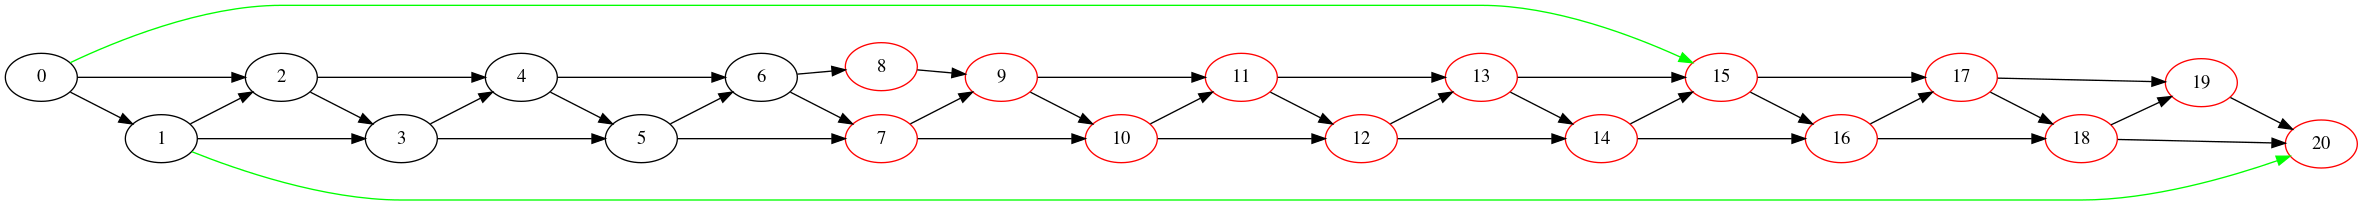
\includegraphics[width=1\textwidth]{bilder/msplit3}
	\end{center}
	\caption{Erster Fall beim Strangaufbau}
	\label{msplit}
\end{figure}

Als erstes behandeln wir Fälle, wie den in Abbilung \ref{msplit} dargestellten Fall. Der abgebildete Graph ist aus der im letzten Kapitel erläuterten Methode entstanden. Die roten Knoten sind die Contigs aus $P_V$, die schwarzen Knoten sind die Contigs $P$, welche Constraints nach $P_V$ aufweisen. Die Knoten wurden nach ihrer Position durchnummeriert und entsprechend benannt. 
% A19: Die Zahl an den Kanten gibt die Anzahl an Constraints an, welche die Kante unterstützen. + nächster Satz ergänzt
Die grünen Kanten stellen auch hier wieder die nicht verlängerbaren Kanten dar.
%Grüne Kanten sind Kanten, bei denen sowohl Anfangsknoten wie auch  Endknoten keine Constraints zu weiter entfernten Constraints aufweisen


$S_0$ besteht aus den beiden Contigs 7 und 8. Für ein Grundgerüst der DNA ist es egal, mit welchem der beiden Contigs weitergearbeitet wird. Daher werden in einem Fall, bei denen von zwei Contigs aus $S_0$ die gleichen Contigs erreicht werden können, immer der Contig aus $S_0$ entfernt, welcher mit den meisten fest positionierten Contigs erfüllte Constraints aufweist. 
% A19: In diesem Fall wäre es Contig 7, da Contig 8 nur eine einlaufende Kante von 6 aus hat, wohingegen Contig 7 mindestens zwei einlaufende Kanten hat (wahrscheinlich hat 7 aber auch von den restlichen vorherigen Contigs einlaufende Kanten).
In diesem Fall fällt die Wahl auf Contig 7, denn Contig 8 besitzt insgesamt nur eine einlaufende Kante (ansonsten wären in dem Graphen mindestens zwei Kanten sichtbar eingezeichnet), während Contig 7 mindestens zwei einlaufende Kanten besitzt. Dabei ist zu beachten, dass in unserer Darstellungsform nicht alle vorhandenen Constraints eingezeichnet werden, um eine Übersichtlichkeit zu ermöglichen. Damit können für Contig 7 noch weitere Kanten existieren, die ebenfalls hier berücksichtigt werden. 
%Dies ist auch sehr wahrscheinlich, da es eine nicht verlängerbare Kante von Contig 1 zu Contig 20 gibt. 


\begin{figure}
	\begin{center}
		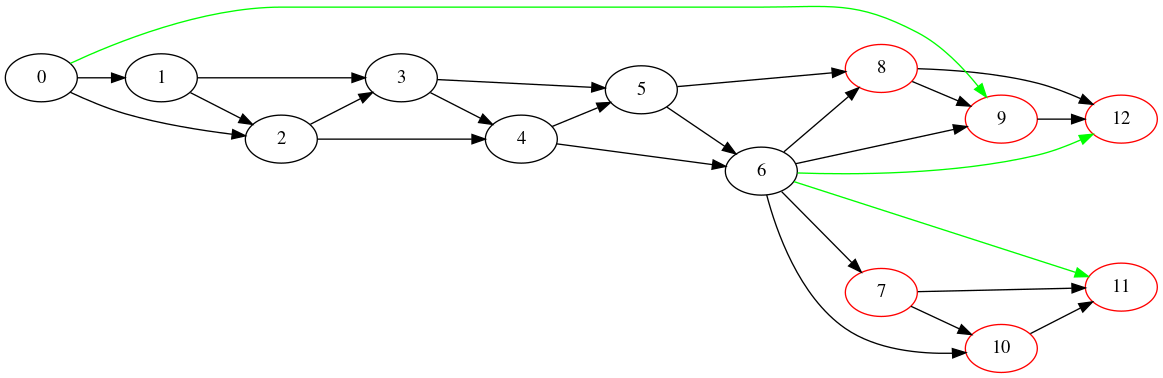
\includegraphics[width=1\textwidth]{bilder/bigsplit}
	\end{center}
	\caption{Beispiel für einen weiter Situation, die beim Strangaufbau auftreten kann}
	\label{bigsplit}
\end{figure}
Nun nehmen wir uns die restlichen Fälle vor, bei denen eine falsche Entscheidung gravierende Auswirkungen haben könnte. Ein Standardbeispiel ist in Abbildung \ref{bigsplit} dargestellt. 
% A19 : modifizierter nächster satz
Die Menge aus Contig 7, 10 und 11, hat ausschließlich eine Kante zu Contig 6, während die Menge aus 8, 9 und 12 zu sämtlichen vorhergehenden Contigs Kanten hat.
Dies ist auch anhand der Abbildung ersichtlich. Zwar sind nicht alle besagten Kanten eingezeichnet, jedoch ist bekannt, dass alle schwarzen Contigs zu mindestens einem roten Contig eine Kante besitzen. Anhand der grünen, also nicht verlängerbaren Kante von Contig 6 zu Contig 11 und dem Fehlen weitere einlaufender, grüner Kanten in die Menge $\{ 7, 10, 11 \}$ sieht man, dass es keine weiteren Kanten ausgehend von den schwarzen Contigs geben kann. Ansonsten müsste eine weitere nicht verlängerbare Kante vorhanden sein.
Per Ausschlussprinzip folgt so ebenfalls, dass die verbleibenden schwarzen Contigs mindestens eine in die Menge $\{8,9,12\}$ einlaufende Kante besitzen.

% A19: Modifizierungen beim Absatz
Die typische Situation bei einem Repeat ist, dass es aus der Repeat-Region, die auch aus mehr als einem Contig bestehen kann, Constraints zu allen Abzweigungen gibt. Aber nur zu einer Abzweigung gibt es Constraints, die vom Abschnitt vor der Repeat-Region kommen. Dies untersuchen wir als erstes.

Wir ordnen jedem Element $s$ aus $S_0$ jene Knoten aus $H$ zu, welche ausschließlich von $s$ erreicht werden können und bezeichnen die Menge dieser Knoten mit $V_s$ (es gilt stets $s \in V_s$). Nun erstellen wir für jedes $s$ aus $S_0$ eine Menge $P_s$ aus Contigs in $P$, welche Constraints in $V_s$ aufweisen. Die $P_s$ Mengen schneiden wir (der Schnitt ist nicht leer da $a^*$ immer enthalten ist) und ermitteln den Contig $l$ mit der niedrigsten Position aus dem Schnitt. Schließlich berechnen wir für jedes $s \in S_0$ die Anzahl $k_s$ der Contigs aus $P_s$, welche vor $l$ liegen. Sollte für ein $\hat{s}$ aus $S_0$ gelten, dass $k_{\hat{s}} \geq 2k_s+1$ für alle anderen $s \in S_0$ gilt, so ist dies ein deutliches Zeichen, dass  $\hat{s}$ der nächste Contig ist. 


\begin{figure}
	\begin{center}
		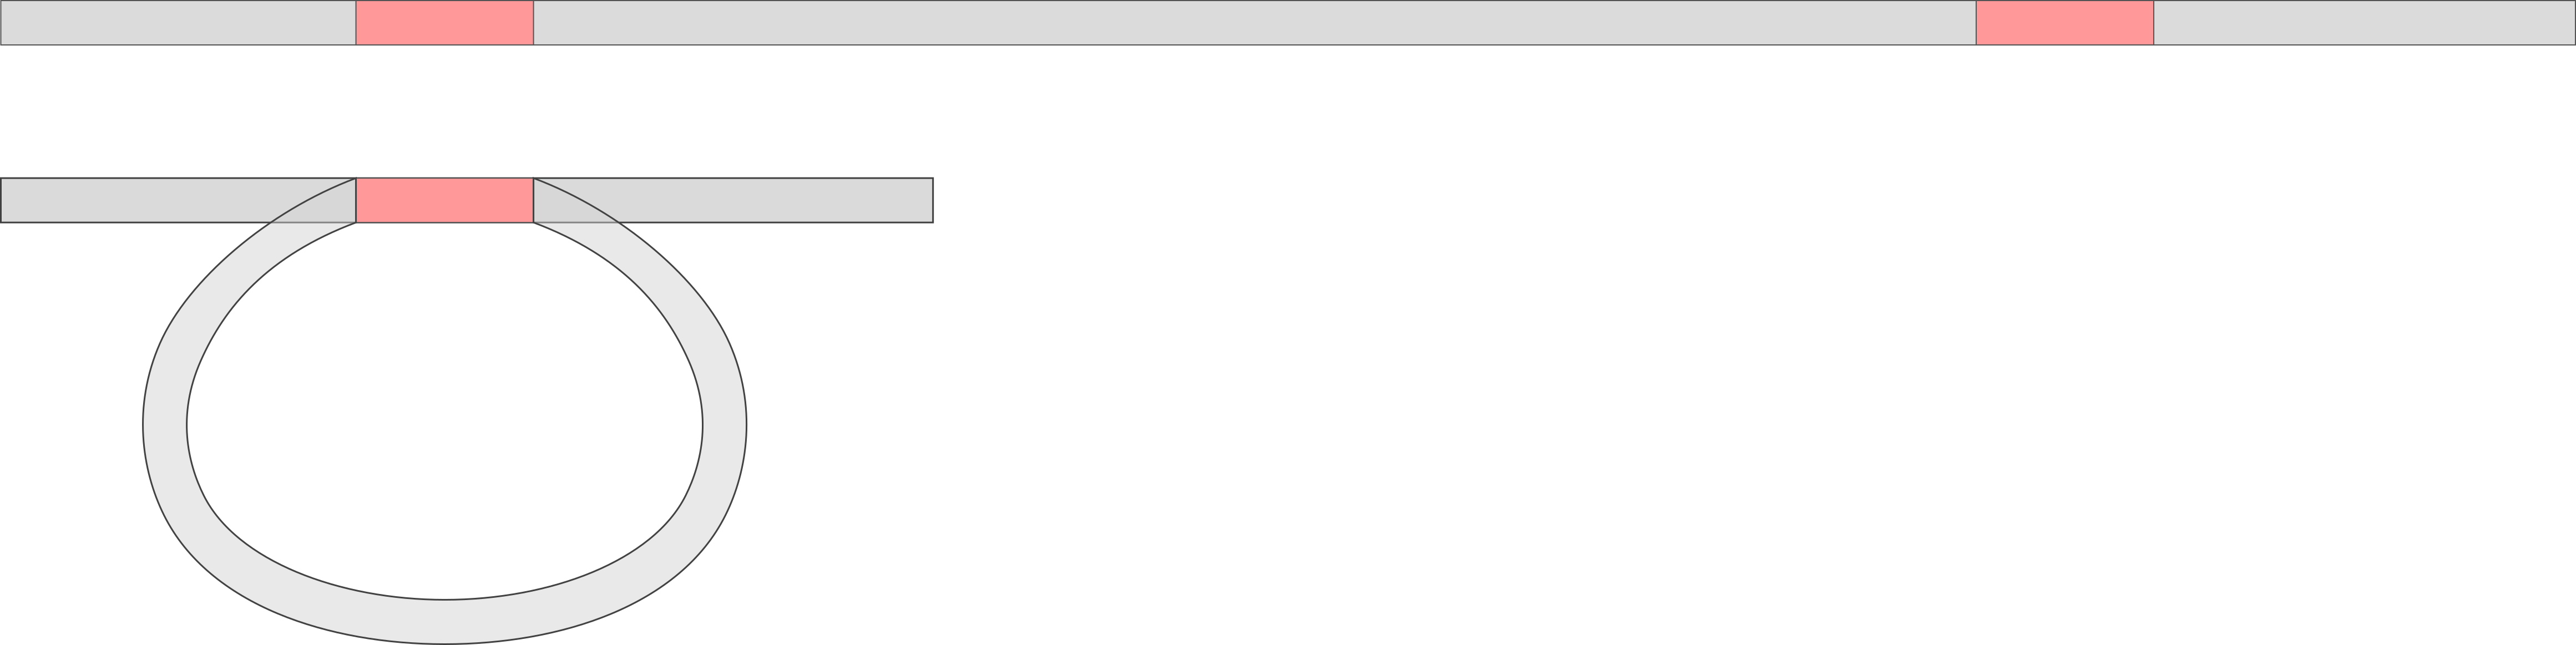
\includegraphics[width=1\textwidth]{bilder/repeat_kreis}
	\end{center}
	\label{repeat_kreis}
	\caption{Repeat in den Daten}
\end{figure}
Sollte dies nicht der Fall sein, so wird noch ein zweiter Aspekt betrachet. Wie in Abbildung \ref{repeat_kreis} angedeutet, erzeugt ein Repeat in den Daten einen Kreis in dem dazugehörigen Graphen. Befinden wir uns gerade im roten Abschnitt und haben den Kreis noch nicht durchlaufen, so sollten wir zuerst dem Kreis folgen. Wenn wir den Kreis durchlaufen haben, können wir immer noch den anderen Abzweig nehmen.

Leider sind diese Kreise nicht so eindeutig zu identifizieren. 
% A19:
Ein Problem tritt auf, falls ein Constraint von einem der letzten Contigs im Strang zu einem der ersten Contigs im Stang geht und damit jeder Contig von jedem anderen aus erreichbar ist. Somit kann man nicht einfach nach einem Kreis in $G$ suchen. Daher schränken wir $G$ auf die Knoten ein, die nicht in $P$ liegen und suchen dann $s_1,s_2 \in S_0$, sodass es einen Weg von $s_1$ nach $s_2$ gibt, aber keinen Weg von $s_2$ nach $s_1$. In so einem Fall entfernen wir $s_2$ aus $S_0$.

% A19:
Sollten wir es geschafft haben, uns auf einen Pfad festzulegen, so wird dieser gewählt, ansonsten werden alle Pfade, die noch nicht ausgeschlossen werden konnten, nacheinander ausprobiert und deren Lösungen gesammelt zurückgegeben.

Wenn es keine weiteren Contigs gibt und die Länge von dem Strang im erlaubten Bereich ist, so wird die Lösung zurückgegeben.

Gibt es mehr als eine Lösung, so werden die Lösungen anhand der Anzahl der verwendeten Contigs verglichen. 

Wir schauen nun, wie die Lösung bislang aussieht. An 81 Stellen haben sich die Contigs aufgeteilt. In allen Fällen konnten die Heuristiken aber einen eindeutigen Pfad identifizieren. Das Ergebnis ist 4\,902\,942 Basenpaare lang und beinhaltet 2106 von 2117 Contigs. Es wurden dabei 55 Repeats vergeben. Diese erfüllen teilweise nicht die Anforderungen an Repeats, welche wir in der Formalisierung festgelegt haben und werden in der nächsten Phase gründlich überprüft.


\chapter{Algorithmus Phase 2: Lösung mithilfe vom LP verfeinern}
Wir haben jetzt bereits einen groben Aufbau und wollen diesen verbessern. Dazu werden wir einen Teil der Contigs mithilfe des LPs setzen, während der andere Teil fixiert bleibt. Schließlich werden wir für jeden Contig schauen, wie er umpositioniert werden müsste, um seine Constraints gut zu erfüllen und wir ermitteln mithilfe einer Gütefunktion, ob und wo der Contig Repeats hat. Dieser Prozess wird mehrfach wiederholt, bis alle Kriterien an eine guten Lösung erfüllt sind.

% A21: Wir überprüfen, ob der zu den Daten gehörende Graph zusammenhängend ist, und werfen Contigs raus, welche nicht erreichbar sind. 
Wir betrachten zunächst den Graphen, der durch die Interpretation der Contigs als Knoten und der Constrainst als gerichtete Kanten ensteht. In diesem werden die schwachen Zusammenhangskomponenten und deren Kardinalität bestimmt und daraufhin alle Contigs gelöscht, die nicht zur größten Komponente zählen.
Weiterhin werden Constraints aus den Daten entfernt, wenn sie zwei gleiche Contigs beinhalten und die Distanz kleiner als 1\,000 ist, da wir aufgrund der Toleranz von 500 Basenpaaren keine Repeats auf so kleiner Entfernung finden können.

Um unsere Lösung aus dem vorherigen Teil verwenden zu können, müssen wir das Lineare Programm anpassen. Dafür modifizieren wir die Positionen leicht und erstellen eine Menge aus Contigs, deren Positionierung als richtig angenommen werden kann. Dies funktioniert wie folgt:


Für die Neupositionierung benutzen wir ein ähnliches Verfahren wie beim letzten Kapitel. Wir erstellen zuerst für jeden Contig eine leere Liste
und fügen für jeden Constraints $(a,b,d)$ den Wert $\pos(a)+d$ in die Liste von $b$ und den Wert $\pos(b)-d$ in die Liste von $a$ ein. Sollte Contig $a$ als ein Repeat mit Versionen $a_1$, $a_2$, ..., $a_n$ vorgemerkt sein, so werden für Contig $b$ die Werte $\pos(a_1)+d$, $\pos(a_2)+d$, ..., $\pos(a_n)+d$ gespeichert und es wird vermerkt, dass diese Positionen von einem Repeat stammt. 
Zu Beginn stammen potentiellen Repeats aus dem Verfahren des vorherigen Kapitels. 
Ist Contig $b$ ein Repeat, so wird analog verfahren.
Zusätzlich wird zu jeder Position in den Listen noch der jeweils andere Contig aus dem korrespondierenden Constraint und die Information, ob dieser Constraint einlaufend oder auslaufend ist, gespeichert.

Die Positionen werden gruppiert, indem Positionen, welche weniger als 500 Basenpaare auseinanderliegen, zusammengefasst werden und dann der Median berechnet wird. Die Mediane werden nun mit zwei Güten ausgestattet. 

Diese Güten berechnen sich aus den folgenden Werten:
\begin{itemize}
	% A21 : leichte Modifikationen
	\item[$i$:] 1, falls sowohl auslaufende als auch einlaufende Constraints beteiligt waren; \\ 0 sonst;
	\item[$h$:] das Vorkommen des am häufigsten auftretenden Contigs;
	\item[$a$:] die Anzahl an Positionen;
	\item[$m$:] die Anzahl an Positionen, welche nicht von Repeats stammen;
	\item[$p$:] $150 / (100+s)$, wobei $s$ die Standardabweichung ist.
\end{itemize}

% A21: kleinere Modifikationen in dem Abschnitt; Formel jetzt in Umgebung
Mithilfe der ersten Güte $g_0$ soll entschieden werden, an welchem Ort sich der Contig befindet. Sie berechnet sich durch 
\[  g_0 = a\ (\log_2(h) + 0.5) \ (0.5i + 0.5)\  p . \]
Dies erklärt sich wie folgt: Die Gruppengröße, also die Anzahl an Constraints, die den Contig an dieser Position sehen, ist der wichtigste Indikator. 
Es können aber mehrere Constaints aus dem selben Long-Read stammen. Wenn dieser fehlerhaft ist, so wären eventuell alle Constraints aus diesem Read falsch. Der Wert $h$ gibt an, von wie vielen verschiedenen Long-Reads die Constraints mindestens stammen. Daher bestrafen wir die Positionen mit $h=1$ und belohnen Positionen, für die $h$ groß ist. 
Weiterhin ist eine Position zu bevorzugen, bei der ein Contig sowohl einlaufende als auch auslaufende Constraints hat. Zuletzt deutet eine kleinere Standardabweichung auf eine größere Sicherheit der Position hin. 

% A21: Mittels der zweiten Güte $g_r$ soll entschieden werden, wo der Contig einen Repeat besitzt. Die zweite Güte beachtet also die strengeren Anforderungen an einem Repeat. Diese ist 0 sobald $h \leq 2$ oder $i = 0$ oder $s = 0$, ansonsten berechnet sie sich durch $g_r = s\ \log_2(h) \  p$.

% A21: umgeschrieben
Mittels zweiten Güte $g_r$ soll entschieden werden, an welchen Stellen der Contig einen Repeat besitzt. Die zweite Güte beachtet also die strengeren Anforderungen an einem Repeat. 
% A21: Diese ist 0 sobald $h \leq 2$, ansonsten berechnet sie sich durch $g_r = s\ \log_2(h) \ i \  p$.
Sie berechnet sich wie folgt:
\[ g_r = \left\{
\begin{array}{ll}
0 & \textrm{falls } h \leq 2 \\
m\ \log_2(h) \ i \  p & \, \textrm{sonst.} \\
\end{array}
\right. \]

% A21: Hier werden also die Constraints von einem Repeat nicht zu Anzahl gezählt
Anstatt der Gesamtheit an Positionen betrachten wir also hier mittels $m$ nur die Positionen, die nicht von Repeats stammen.
%, das liegt daran, dass ein Contig, der ausschließlich Constraints mit  Repeats besitzt, wahrscheinlich bei der anderen Repeat-Version anzusiedeln ist
% A21: und es muss einlaufende und auslaufende Constraint geben sowie einen mindestens dreifach abgesicherter Constraint dabei sein. 
Ferner wird sichergestellt, dass sowohl einlaufende als auch auslaufende Constraints beteiligt sind, sowie dass mindestens ein dreifach abgesicherter Constraint dabei ist. 
Dadurch werden alle Anforderungen der Formalisierung erfüllt.

% A21: bisschen Grammatik und Rechtschreibung, sowie g_r >= 300
Nach der Berechnung der Gütewerte wird jedem Contig die Position mit dem größten $g_0$ zugeordnet, außer es gibt Positionen bei denen $g_r$ größer als ein Schwellwert ist, welcher zu Anfang bei 300 liegt. In diesem Fall wird für jede Position mit $g_r \geq 300$ eine Version des Contigs erstellt.

% A21: Constraints -> Bedingungen; erster Schritt -> Phase 1
Jeder Contig mit $g_0 > 50$ gilt als sicher. Bei diesen Contigs wird die Position als Konstante in den Bedingungen des LPs gesetzt und es werden nur die Positionen der als unsicher geltenden Contigs durch das LP bestimmt, sowie der Contigs, die in Phase 1 nicht positioniert wurden. Bevor das LP ausgeführt wird, müssen noch die Constraints auf die Repeat-Versionen verteilt werden. 
%Dabei wird ein Constraint $(a,b,d)$ allen Kombinationen von Contig $a$-Repeats mit Contig $b$-Repeats zugeordnet, für die sein Fehler kleiner als 1\,000 ist.
Dabei wird ein Constraint $(a,b,d)$ all jenen Repeat-Versionen zugeordnet, für die der Constraint erfüllt ist. Wird ein Constraint von keinem Repeat erfüllt oder wurde einer der beiden Contigs im Repeat noch nicht positioniert, so wird der Constraint allen Versionen zugeordnet.

Für die Feinpositionierung lassen wir ein zweites LP mit den glaubwürdigsten Constraints laufen. Dabei wird ein ähnlicher Graph wie bei Plotten erzeugt. Die ersten drei Punkte sind identisch, aber es werden andere Kanten verwendet:
\begin{itemize}
	\item Zunächst werden alle Constraints gelöscht, deren Fehler in der vorgegebenen Positionierung größer als 2\,000 ist.
	\item Ferner werden mehrfach auftretende Constraints zusammengefasst und alle Schleifen, also alle Constraints der Form $(a, a, d)$ gelöscht.
	\item Sei nun $N_a$ die Menge aller Contigs, die zusammen mit $a$ in einem verbliebenden Constraint enthalten sind. Nun werden die Contigs in $N_a$ und $a$ selbst bezüglich ihrer Positionierung sortiert.
	\item Schließlich erhält jeder Contig fünf auslaufende Kanten zu den Nachfolgern, die am meisten gemeinsame Constraints mit ihm aufweisen. Sollte ein Gleichstand auftreten, wird die Sortierung aus dem vorherigen Unterpunkt beachtet und nahliegende Contigs werden bevorzugt. Analog erhält der Contig fünf einlaufende Kanten ausgehend von fünf seiner Vorgänger.
	% A21: Schließlich werden für jeden Contig Kanten von den fünf Vorgängern gezeichnet, welche am meisten Constraints mit ihm aufweisen, analog  mit den Nachfolgern. Bei gleich vielen Constraints wird die Vorsortierung aus dem letzten Schritt beachtet, und nah ligende Contigs bevorzugt.
\end{itemize}
Nun werden alle Constraints gesammelt, die eine Kante in dem Graphen darstellen und ausschließlich diese Constraints werden als Bedingungen in dem LP verwendet.
% A21: Zusätzlich werden die Contigs alle nach ihrer Position sortiert und es wird ein Constraint zu je zwei Nachbarn mit ihrer aktuellen Entfernung eingefügt. Dadurch ist sichergestellt, dass die Daten noch zusammenhängend sind. 
Zusätzlich werden die Contigs nach ihrer aktuellen Position sortiert. Für je zwei benachbarte Contigs (gemäß der Sortierung) fügen wir einen weiteren Constraint ein, welcher als Distanz die aktuelle Entfernung der Contigs besitzt. Dadurch soll sichergestellt werden, dass die Daten noch zusammenhängend sind.

Leider kann es passieren, dass das LP größere Schwierigkeiten hat, eine Lösung zu finden. Dies passiert, wenn Bereiche der Daten durch nur sehr wenige Constraints verbunden sind und macht sich bemerkbar durch die folgende Meldung von Gurobi: 

% A21: Hab's mal kursiv gemacht
\textit{„Numerical trouble encountered\\
	\\
	Model may be infeasible or unbounded.  Consider using the\\
	homogeneous algorithm (through parameter 'BarHomogeneous')“}

Daher wurden noch zusätzliche Constraints eingefügt, die den Lösungsraum auf einen sinnvollen Bereich einschränken. Dies geschieht, indem jeder Fehler um maximal 2\,000 Basenpaare abweichen darf. Eine stärkere Abweichung ist unrealisch, wenn davon ausgegangen wird, dass die bisherige Lösung nicht komplett falsch ist.

% A21: Modifikationen
Dieser Vorgang wird nun wiederholt. Es werden für alle Contigs Positionen mit Gütewerten berechnet, abhängig von der Güte Repeats erzeugt und mithilfe der beiden LPs die Positionen angepasst. Dabei können auch schon zuvor erstellte Repeats wieder entfernt werden. Bei jedem Durchlauf wird der Schwellwert für $g_r$ verringert, sodass schrittweise mehr Repeats zugelassen werden.
% A21: ab der ein Repeat vergeben wird. 
Wie stark die Grenze reduziert wird, hängt von der Anzahl an gefundenen Repeats ab. Wurden viele Repeats gefunden, so wird die Grenze gar nicht bis kaum verändert. Werden jedoch keine Repeats gefunden, so wird die Grenze stark reduziert. Es sei $n$ die Anzahl der neu hinzugekommenen Repeats und $s_0$ die alte Schranke. Dann berechnet sich die neue Schranke $s_1$ durch:
\[ s_1 = \frac{s_0}{1 + 0.2\frac{5 - n}{5}}\]

Das Program wird beendet, sobald die Schranke unter 10 fällt.

% A21: Die Kannt
% A21: welcher auch für des plotten verwendet wir. Es werden aber keine Grünen kannten verwendet und vier einlaufenden und auslaufenden Kanten. Diese KanteNur Constraint die zu einer Kante in diesem Graphen korrespondieren, werden verwendet. Hintergrund ist, dass je weiter Contigs auseinanderliegen, desto größer ist der zu erwartende Fehler. Daher werden nur Constraints von den nahen Contigs berücksichtigt.


\chapter{Auswertung der Ergebnisse}
An dieser Stelle wollen wir nun kurz die Ergebnisse unserer Arbeit zusammenfassen.
Zu Beginn hatten wir einen Lösungsversuch gestartet, bei dem nur ein einziges lineares Programm verwendet wurde.
Dieses hat jedoch noch keine Repeats berücksichtigt, was in einem teilweise ineinander verflochtenem Lösungsstrang resultierte.

Daraufhin wurde ein neuer Ansatz verwendet. Die Idee war es, in zwei Phasen zu arbeiten.
In der ersten Phase kam noch kein lineares Programm zum Einsatz. 
Stattdessen wurde zunächst ein Grundgerüst in Form eines Pfades konstruiert, bei dem Repeats bereits zum Teil berücksichtigt wurden.
Teilweise erfüllen diese Repeats unsere Anforderungen aber nicht.
In der zweiten Phase wird dies genauer unter die Lupe genommen. 
Mittels selbst konstruierter Gütefunktionen werden hier neue Repeats gesetzt, „unsichere“ Repeats gelöscht und weiter Contigs in den Strang eingefügt.
Das Positionieren der Contigs und der Repeats übernehmen zwei lineare Programme. 
Die Idee hinter dem ersten Programm war es, falsch positionierte Contigs neu zu setzen, indem man „sichere“ positionierte Contigs in dem Programm fixiert.
Das zweite Programm diente der Feinpositionierung. Hier wurde die Anzahl Bedingungen reduziert, indem „unsichere“ Constraints verworfen wurden. 
Eine Grafik von dem zugehörigen Graphen des Ergebnisses nach der zweiten Phase findet man in dem zugehörigen Githup Repository unter dem Namen „lösung.png“.


Nun werden wir uns kritisch mit dieser Lösung auseinander setzen. Zunächst einmal positiv anzumerken ist, dass die starken Verflechtungen aus dem ersten Ansatz eliminiert werden konnten.

Die finale Stranglänge beträgt 4\,902\,231 Basenpaare und passt somit zu der erwarteten Gesamtlänge, sodass der vierte Anforderungspunkt erfüllt ist. Der erste Anforderungspunkt an unsere Lösung besagt, dass abgesicherte Constraints möglichst alle beachtet werden sollten.
Überprüft man in der Lösung alle abgesicherten Constraints, so findet man 35 Constraints, die in der Lösung nicht erfüllt sind. Die genaue Anzahl hängt aber aber auch von der Toleranz ab, die man verwendet (hier 1000). 
Wenn man diese etwas lockert (auf 3000), werden noch 27 nicht erfüllte, abgesicherte Constraints gefunden. Dabei werden Dopplungen nicht mit einberechnet.
Es gibt jedoch vier Contigs, von denen jeweils mindestens ein Contig in den 27 Constraints involviert ist.

Eine Möglichkeit wäre das Hinzufügen weiterer Repeats für diese Contigs.

(Von den insgesamt 143\,630 Constraints sind 75\,774 nicht abgesichert (mit Dopplungen).)

Insgesamt sind rund 97,87\% der Constraints erfüllt. Offenbar ist somit also gemäß des zweiten Anforderungspunkt auch ein Großteil der verbleibenden, nicht abgesicherten Constraints erfüllt.

Ferner wollten wir, dass es vermieden wird, Contigs ohne gemeinsame Constraints nah beieinander zu positionieren.

Wir betrachten nun die finale Lösung, schauen uns alle Paare von benachbarten Contigs an und zählen die Anzahl an Paare, die keinen gemeinsamen Constraint besitzen.

Insgesamt findet man so 14 Paare, die diese Bedingung verletzen.

Wenn man gemäß der Beobachtungen beim ersten Anforderungspunkt noch weitere Repeats hinzufügt, steigt diese Anzahl weiter an.

Eine zukünftige Herausforderung wäre es, zu untersuchen, ob es möglich ist, diese Lücken in den Constraints durch ein anderes Assemblierungsverfahren zu vermeiden oder ob es sich hierbei um ein Problem in den Daten selbst handelt.

Besonders sollte man dabei die Paare beachten, die ansonsten, zum Beispiel anhand der definierten Güte $g_0$, gut in den Strang eingebunden sind.


Wir hatten bereits erwähnt, dass die Länge des finalen Stranges zu den Vorgaben aus dem vierten Unterpunkt passt.

Zu erwähnen bleibt hier aber noch, dass die finale Länge abhängig davon ist, welche Constraints bei der Feinpositionierung betrachtet werden.


Verwendet man hauptsächlich relativ kurze Constraints (also Constraints zwischen fast unmittelbaren Nachbarn), so wird die Gesamtlänge größer und es kann in Kombination mit dem restlichen Programm passieren, dass der Strang auseinander reißt. Verwendet man sehr lange Constraints, so wird der Strang etwas kürzer. Auch hier kann es passieren, dass der Strang auseinander reißt. Eine weitere Herausforderung wäre es, dies genauer zu untersuchen. Eine mögliche Ursache wäre ein systematischer Fehler in den Daten.

Schließlich bleibt noch der letzte Unterpunkt der Anforderungen, welcher besagt, dass eine Aufteilung des Ergebnisses in „sichere“ und „unsichere“ Gebiete erwünscht sei.

Hier kann man beispielsweise die Gütefunktionen zu Rate ziehen.


Insgesamt gibt es 53 Contigs mit $g_r = 0$.

Davon haben 22 Contigs eine Güte $g_0$, die kleiner als 10 ist.

Diese sind offenbar sehr unsicher und es ist wahrscheinlich nicht sinnvoll, sie in eine Lösung mit aufzunehmen. 

Die verbleibenden 31 Contigs mit $g_0 \geq 10$ passen mit hoher Wahrscheinlichkeit ebenfalls nicht so gut in ihre Nachbarschaft. Ein Grund dafür könnte jedoch auch die Nachbarschaft selbst sein, wodurch die Bereiche rund um diese Contigs zu unsicheren Gebieten zählen und näher betrachtet werden sollten.


Ähnlich lassen sich so auch „sicher“ Gebiete lokalisieren.

Die Forderung $g_r \geq 50$ wird von rund 92,7\% der Contigs erfüllt. Diese würden wir zu den tendenziell sicheren Gebieten zählen.
\chapter{Diskussion}
Die LPs haben in diesem Verfahren nur eine untergeordnete Aufgabe. Mithilfe von ILPs könnte man auch versuchen, die erste Phase zu lösen.
So könnte man einen Weg von dem Anfang des Strangs bis zum Ende suchen, der möglichste viele Constraints erfüllt. 
Dies könnte so aussehen: Sei $D$ die Menge der Contig-Paare, welche einen gemeinsamen Constraint besitzen.

\begin{align*}
\text{Integer-Variablen:}\quad& e_{a,b} &\forall (a,b) \in D\\
\text{Zielfunktion:}\quad& \max \sum_{(a,b) \in D} e_{a,b}\\
\text{Bedingungen:}\quad& \sum_{(a,b) \in D} e_{a,b} = \sum_{(b,c) \in D} e_{b,c} &\forall b \in C-\{s,t\}\\
& \sum_{(a,s) \in D} e_{a,s}+1 = \sum_{(s,c) \in D} e_{s,c}\\
& \sum_{(a,t) \in D} e_{a,t} = \sum_{(t,c) \in D} e_{t,c} +1
\end{align*}

Die Bedingungen sorgen dafür, dass sich für jeden Knoten die einlaufenden und auslaufenden Kanten ausgleichen. Damit dies ein Pfad wird, muss noch der Zusammenhang sichergestellt werden. Dies kann mit 0-1-Variablen realisiert werden, die für jede Teilmenge der Knoten, die den Startknoten $s$ nicht enthält, dafür sorgen, dass wenn ein Kante innerhalb der Knotenmenge liegt, es auch eine einlaufende Kante in die Knotenmenge gibt:

\begin{align*}
\text{0-1-Variablen:}\quad& x_V &\forall V \subset C-\{s\}\\
\quad& y_V &\forall V \subset C-\{s\}\\
\text{Bedingungen:}\quad&  x_V \leq \sum_{(a,b) \in D \cap (V \times V)}  e_{a,b} \leq |D| x_V  &\forall V \subset C-\{s\}\\
\quad&  y_V \leq \sum_{(a,b) \in D \cap ((C-V) \times V)}  e_{a,b} \leq |D| y_V  &\forall V \subset C-\{s\}\\
\quad&  x_V \leq y_V  &\forall V \subset C-\{s\}
\end{align*}

Die Variable $x_V$ ist 0 genau dann, wenn es keine Kante in $V$ gibt. Die Variable $y_V$ ist 0 genau dann, wenn es keine Kante von $C-V$ in $V$ gibt.
Dies sind viel zu viele Bedingungen, um sie alle zu definieren. Man kann aber das Program ohne diese Bedingungen durchlaufen lassen und schrittweise Bedingungen hinzufügen, welche in der Lösung verletzt wurden und das ILP neu ausführen.

Weiterhin würden viel zu viele Schleifen eingfügt werden, wenn alle Constraints beachtet werden würden, daher wird eine transitive Reduktion durchgeführt, welche die Distanzwerte beachtet. Eine Kante wird also entfernt, wenn es einen Weg vom Start zum Endknoten aus kürzeren Kanten gibt, deren Distanzen sich auf die Distanz der längeren Kante aufsummieren (natürlich wieder mit Beachtung einer Fehlertoleranz).

Diese Kantenreduktion entspricht im Prinzip einer minimalisierten Version des Anfangsproblems, wenn wir einen Constraint vom ersten zum letzten Contig im DNA Strang hinzufügen mit der ungefähren Distanz von 4\,900\,000 Basenpaaren. Aber wie auch bei den grünen Kanten in der Graphdarstellung, reicht es für gewöhnlich aus, Wege der Länge 2 zu überprüfen.

Ein weiteres Problem ist das Ablesen der Lösung aus dem LP. Im Grunde liefert das LP nur eine reduzierte Version des Graphens. Um die Lösung zu erhalten, muss noch ein Eulerweg durch den Graphen gefunden werden. Dies ist aber kein schweres Problem und networkx bietet einen Algorithmus für Eulerkreise.

Es bleibt aber das Problem, dass es für das LP besser ist, 1\,000 Repeats zu erzeugen, wenn dadurch nur eine Kante zusätzlich aufgenommen werden kann. Daher müsste man Repeats bestrafen. 

Dies könnte man machen, indem eine einfache Kante belohnt, eine Mehrfachkante aber bestraft. Denkbar wäre eine Realisierung mittels zusätzlicher 0-1-Variablen, die den Wert 1 besitzen, sobald eine Kante einmal verwendet wird:

\begin{align*}
\text{0-1-Variablen:}\quad& e'_{a,b} &\forall (a,b) \in D\\
\text{Bedingungen:}\quad& e'_{a,b} \leq e_{a,b}&\forall (a,b) \in D\\
\text{neue Zielfunktion:}\quad& \max \sum_{(a,b) \in D} (5 e'_{a,b} - e_{a,b})
\end{align*}

Theoretisch ist ein solches ILP interessant, jedoch ist die Laufzeit der entscheidende Nachteil. Aufgrund der Vielzahl an Bedingungen und der ohnehin schon langen Laufzeit pro Durchlauf ist die Realisierung nicht sehr praktikabel.
\backmatter
%% Anhang - Wenn kein Anhang erstellt werden soll, dann lassen Sie diese Datei einfach leer.

\begin{appendix}
\appendix
\chapter{\appendixname}


z.B. eine CD mit Quelltexten o.\"a.


\end{appendix}

%\renewcommand*{\bibname}{References}
\bibliography{quellen}

%\bibliographystyle{alphadin}
\bibliographystyle{abbrvdin}




%\addcontentsline{toc}{chapter}{\listfigurename}
\cleardoublepage

\chapter{Ehrenw\"ortliche Erkl\"arung}

Hiermit versichere ich, die vorliegende \Typ \ selbstst\"andig verfasst und keine anderen als die angegebenen Quellen und Hilfsmittel benutzt zu haben.\\

\noindent Alle Stellen, die aus den Quellen entnommen wurden, sind als solche gekennzeichnet.\\

\noindent Diese Arbeit hat in dieser oder \"ahnlicher Form noch keiner Pr\"ufungsbeh\"orde vorgelegen. \\

\vspace{8cm}
\noindent D\"usseldorf, 13. August 2019%\today
\begin{flushright}
$\overline{\text{~~~~~~~~~~~~~~~~~~~~~~~~~~~~~~~~~~~~~~~~~~~\Autor}}$
\end{flushright}
%\cleardoublepage

\end{document}
